\documentclass[12pt,a4paper]{report}

% ---------------- Packages ----------------
\usepackage[utf8]{inputenc}
\usepackage[T1]{fontenc}
\usepackage{polyglossia}
\setmainlanguage{english}
\usepackage{fontspec}
\newfontfamily\nepalifont{Noto Sans Devanagari}[Script=Devanagari,Renderer=HarfBuzz]
\usepackage{float}
\usepackage{graphicx}
\usepackage{amsmath, amssymb}
\usepackage[style=apa, backend=biber, url=true, natbib=true]{biblatex}
\addbibresource{references.bib}
\usepackage{setspace}
\usepackage{geometry}
\usepackage{microtype}
\usepackage{subcaption}
\usepackage{booktabs}
\usepackage{caption}
\usepackage{rotating}
\usepackage{siunitx}
\usepackage{enumitem}
\usepackage{longtable}
\usepackage{pdflscape}
\geometry{a4paper, top=3.5cm, bottom=3cm, left=3.5cm, right=3cm}
\usepackage{fancyhdr}
\setlength{\headheight}{15pt}
\setlength{\headsep}{10pt}
\usepackage{titlesec}
\titlespacing*{\chapter}{0pt}{30pt}{15pt}
\titlespacing*{\section}{0pt}{15pt}{5pt}
\titlespacing*{\subsection}{0pt}{10pt}{5pt}
\titlespacing*{\subsubsection}{0pt}{8pt}{3pt}
\setotherlanguages{hindi}
\newfontfamily\hindifont{Noto Sans Devanagari}[Script=Devanagari]
\sloppy

% Must come after biblatex for clickable links
\usepackage[colorlinks=true, linkcolor=blue, urlcolor=blue, citecolor=blue]{hyperref}

% ---------------- Formatting ----------------
\titleformat{\chapter}[hang]{\huge\bfseries}{\thechapter.}{1em}{}
\setlength{\parskip}{0.5em}
\setlength{\parindent}{0pt}
\onehalfspacing
\pagestyle{fancy}
\fancyhf{}
\rhead{\thepage}
\lhead{Predicting Tiktok Virality in Nepal}

% ---------------- Title Info ----------------
\title{Predicting TikTok virality: Machine learning insights from Nepal’s 2022 election }
\author{Nima Thing}
\date{April 2025}

% Redefine \maketitle for custom title page
\makeatletter
\renewcommand{\maketitle}{
\begin{titlepage}
\thispagestyle{empty}
\onehalfspacing
\setlength{\parskip}{0.5em}
\setlength{\parindent}{0pt}

% Logo in top-right corner
\begin{minipage}{0.3\textwidth}
\raggedleft
\vspace*{1cm}

\includegraphics[width=0.9\textwidth]{figures/hertie_logo.png}
\end{minipage}

% Centered content
\begin{center}
\vspace*{2cm}
{\Large\bfseries\@title \par} % Reduced from \huge to closer to 12pt
\vspace{1.5cm}

{\normalsize\@author \par} % 12pt
\vspace{1cm}

{\normalsize In partial fulfillment of the requirements for the degree of \par}
{\normalsize Master of Data Science for Public Policy \par}
\vspace{0.5cm}

{\normalsize Hertie School \par}
\vspace{0.5cm}

{\normalsize Supervisor: Prof. Dr. Simon Munzert \par}
\vspace{0.5cm}

{\normalsize Academic Year: 2025 \par}
\vspace{0.5cm}

{\normalsize Matriculation Number: 231291 \par}
\vspace{0.5cm}

{\normalsize Word Count: 7694  \par}
\vspace{0.5cm}

{\normalsize\@date \par}
\vspace{1cm}

\end{center}
\end{titlepage}
}
\makeatother

\begin{document}

% ---------------- Roman Numerals for Front Matter ----------------
\pagenumbering{roman}

% ---------------- Title Page ----------------
\maketitle

% ---------------- Executive Summary ----------------

\begin{abstract}
Nepal’s 2022 elections marked a turning point in political communication, with social media platforms such as Facebook, YouTube, and TikTok emerging as a powerful tool for political engagement amid widespread youth disillusionment with traditional parties. Beyond mere platform adoption, virality on TikTok—measured through likes, shares, and comments—became a crucial mechanism for amplifying political narratives and shaping public discourse. 

Despite TikTok’s growing influence, little research has systematically examined how political content achieves virality on the platform, particularly in low-income, multilingual democracies like Nepal. Understanding and predicting virality is not only methodologically innovative—leveraging multimodal machine learning on audio, image, and text data—but also critical for unpacking how digital spaces shape electoral dynamics.

This study analyzes 2,964 political TikTok videos accessed via TikTok’s Research API, applying machine learning (XGBoost) and statistical modeling (OLS regression) to predict engagement outcomes. The XGBoost model achieved approximately 60\% accuracy, identifying sender characteristics as key predictors (mean $|\text{SHAP}| \approx 0.4$), while also revealing algorithmic biases favoring established creators, raising equity concerns. Furthermore, communication styles such as humor and charismatic leadership, particularly when tied to independent political narratives, significantly boosted virality, reflecting Nepal’s culturally diverse digital landscape.

The research provides an open-source multimodal virality prediction pipeline, operationalized engagement metrics, and a cross-platform framework adaptable to platforms like YouTube Shorts. It offers critical insights for political strategists and policymakers aiming to promote equitable online political discourse and strengthen democratic participation in emerging digital democracies like Nepal.
\end{abstract}

% ---------------- Table of Contents ----------------
\clearpage
\tableofcontents

% ---------------- List of Tables ----------------
\clearpage
\listoftables

% ---------------- List of Abbreviations ----------------
\clearpage
\section*{List of Abbreviations}
\addcontentsline{toc}{section}{List of Abbreviations}
\begin{tabular}{ll}
\textbf{Abbreviation} & \textbf{Definition} \\
\hline
API & Application Programming Interface \\
CPN UML & Communist Party of Nepal (Unified Marxist-Leninist) \\
LaBSE & Language-agnostic BERT Sentence Embedding \\
MiniLM & Mini Language Model \\
OLS & Ordinary Least Squares \\
SHAP & SHapley Additive exPlanations \\
TikTok & Social media platform for short-form videos \\
XGBoost & eXtreme Gradient Boosting \\
\end{tabular}

% ---------------- Main Content with Arabic Numerals ----------------
\clearpage
\pagenumbering{arabic}


\chapter{Introduction}
Nepal’s 2022 local and provincial elections (2079 B.S.) marked a significant shift in the landscape of political communication, with TikTok emerging as a prominent platform alongside more established channels such as Facebook and YouTube \parencite{nepalitimes2025}. These platforms increasingly competed for influence, effectively cannibalizing attention and engagement from traditional media as political parties sought to expand their digital reach. One of the most notable developments was the growing use of these platforms as agenda-setting tools, particularly in mobilizing and engaging the country’s youth amid rising disillusionment with legacy political structures \parencite{FPExplainers2024, dahal2023influence}.

Nepal's local election cycle (prior to provincial/federal election), social media platforms, particularly TikTok, significantly amplified grassroots movements and youth-driven political narratives. Independent candidates, such as Balendra Shah (Balen Shah), capitalized on this shift, leveraging platforms to bypass traditional media and party structures \parencite{DW2022NepalElections}. The ``lauro'' (stick) hashtag, symbolizing the independent movement, gained traction, mobilizing voter support \parencite{AnnapurnaExpress2022}. Creators like ``Routine of Nepal Banda,'' with over 1 million TikTok followers, further boosted visibility for progressive candidates \parencite{dahal2023influence}. This new information ecosystem culminated in the unexpected victory of Balen Shah, a rapper without formal political experience, who secured the Kathmandu mayoral seat with 38.6\% of the vote, outpacing major party candidates \parencite{wikipedia2022local}. While three big traditional parties - Nepali Congress and Communist Parties (CPN-UML and CPN-Maoist Centre) retained dominance, alongside their existing visibility on legacy network and social media campaigns, independent candidates, particularly  Balen Shah gained significant visibility on these platforms, mobilizing youth and reshaping public perception outside traditional political frameworks \parencite{DW2022NepalElections}.

TikTok's unique affordances, such as its algorithmic exposure of low-view videos, its automated "for You" page curation, and its built-in creative tools - has separated it from other legacy platforms that rely heavily on pre-existing networks or paid-content promotion \parencite{guinaudeau2022fifteen}. The centrality of TikTok’s algorithm in enabling ``virality-from-nowhere''—unexpected viral success regardless of a creator’s status or affiliation—fundamentally reshapes political communication during elections \parencite{guinaudeau2022fifteen}. As a participatory and remixable platform, TikTok fosters an environment where influence is unpredictable, allowing anyone, from independent candidates to ordinary citizens, to become a political messenger \parencite{guinaudeau2022fifteen}. As global industries have adapted to this logic, even some top Nepalese politicians have also started to engage with TikTok as communicative campaigning tool \parencite{himalayantimes2025oli}. This has given rise to for their followers to position themselves to leverage their own distinctly local style of political messaging, often blending political content with cultural elements like mimicry, humor, and entertainment, which align with communication styles such as Comedic in this study \parencite{umansky2023dances}. 

However, despite TikTok’s rich metadata and increasing API accessibility \parencite{tiktokResearchAPI2025}, there has been little research examining the factors driving political virality through a multimodal lens. TikTok’s role in Nepal—a low-income, multilingual nation with a history of political volatility—remains largely underexplored as a politican communication tool, particularly following its controversial ban in 2023 and reinstatement in 2024 due to concerns over misinformation and digital governance \parencite{lamichhane2024tik, reuters2024tiktok}. In the context of Nepal’s evolving digital democracy, addressing this research gap is essential to understand virality and its association with several forms of TikTok communication forms   during electoral periods. 

This study offers three key contributions:
\begin{itemize}
    \item \textbf{Academic}: It provides a novel and open-source codebase for multimodal virality analysis, filling a gap in computational political communication research in Nepal.
    \item \textbf{Methodological}: It operationalizes virality through a weighted engagement score (combining views, likes, comments, shares, collects) and compares machine learning models (XGBoost, Random Forest) to identify optimal predictive approaches for TikTok data.
\newpage
    \item \textbf{Practical}: By analyzing communication styles, cultural elements, and musical styles (e.g., rap, Nepali folk), it offers actionable insights for political candidates and content creators to enhance audience reach in Nepal’s diverse digital landscape.
\end{itemize}

This research lays the groundwork for future cross-platform virality studies (e.g., TikTok, YouTube Shorts) and provides a framework for candidates to frame election content more effectively, fostering informed digital campaigning in low-income electoral contexts.
\newpage
\section{Literature Review}

The rapid rise of social media has reshaped political communication, offering new avenues for voter engagement, agenda-setting, and grassroots mobilization. In Nepal, where traditional media has long dominated electoral discourse \parencite{dahal2023influence}, platforms like TikTok have introduced novel dynamics, particularly during the 2022 local and federal/provincial elections. This literature review synthesizes research on social media’s role in political communication, TikTok’s emergence as a political platform, virality prediction, and the interplay of communication styles and content themes, identifying critical gaps that this study addresses in the context of Nepal’s evolving digital democracy.

\subsection{Social Media and Political Communication}

Social media platforms have transformed political communication by enabling rapid information dissemination, amplifying user-generated content, and fostering direct candidate–voter interactions \parencite{van2013socialmedia}. \parencite{mcgregor2019socialmediaelections} argue that platforms like Facebook and Twitter (now X) play a significant role in agenda-setting, influencing public perceptions of key issues during election cycles. For instance, studies in Western democracies have shown that social media activity can enhance voter mobilization, with increased engagement (e.g., likes, shares) correlating with higher voter turnout in some contexts \parencite{bode2016campaign}. However, findings are mixed, with \parencite{piatak2021does} noting that online engagement does not always translate into electoral success, particularly in regions with limited digital infrastructure.

In Nepal, social media has become a vital space for political expression, especially among youths frustrated with the country’s history of political volatility \parencite{bhandari2024weaponizing}. \parencite{dahal2023influence} highlight that unorganized groups and individual creators played a significant role in shaping public discourse, often amplifying anti-establishment sentiments. However, much of the research on social media in Nepal remains qualitative, focusing on user perceptions rather than systematic, data-driven analyses of engagement dynamics. 

\newpage
\subsection{Virality Prediction on Social Media}

Predicting virality on social media has been a focus of computational social science, with studies identifying key drivers such as content features, platform dynamics, and sender characteristics \parencite{berger2012viral}. \parencite{SahJordan2025DecodingReddit} used multi-modal features (text, images, user metadata) to predict Reddit Meme virality, where certain temporal features and content layout was quite significant. Additional work include an  explored video-based platforms, with \parencite{nisa2021optimizing} applying XGBoost Learning algorithm to predict YouTube video popularity using visual and audio features, however, here popularity is primarily based on view\_counts. Besides, the study also doesn't formally operationalize virality, but rather exponential spread in short time, which may not fully capture overall virality as an distinct phenomenon. However, TikTok-specific studies on virality prediction on large dataset are even scarce, largely due to data access restrictions and relative novelty on opening up its research API.

In political contexts, virality prediction is particularly complex, as engagement often depends on emotional resonance and cultural relevance \parencite{berger2012viral}. \parencite{ingelstam2023populism} proposed a threshold of 250,000 views for “mildly viral” political content on TikTok, but such metrics lack standardization, especially in non-Western settings like Nepal where audience sizes and engagement patterns differ. Moreover, while APIs like TikTok’s Research API have enabled multimodal analysis in regions like the U.S., EEA, UK or Switzerland \parencite{tiktokResearchAPI2025}, access remains restricted in Nepal, limiting large-scale computational studies. 

\subsection{Communication Styles and Content Themes}

The interplay between communication styles and content themes is a critical driver of engagement on TikTok, particularly in political contexts \parencite{umansky2023dances}. \parencite{schellewald2021communicative} identified styles such as Comedic, Communaal, and Meta on TikTok, noting that humorous content often garners higher engagement due to its emotional appeal. In political settings, \parencite{cseri2024masterarbeit} found that styles like Charisma/Leadership—often through personalization and visuals rhetoric elicit higher engagement metrics. Styles like Critique/Frustration also resonate with audiences by amplifying anti-establishment sentiments, a trend observed in Nepal’s 2022 elections \parencite{dahal2023influence}.
\newpage
However, existing codebooks for TikTok communication styles \parencite{umansky2023dances} are often Western-centric, lacking cultural specificity for contexts like Nepal. Nepalese political content frequently incorporates local elements, such as mimicry, folk music, and rap, reflecting the country’s linguistic and cultural diversity. For instance, independent candidates like Balen Shah promotional campaign was mostly rap/hiphop to connect with youth voters, blending political themes with entertainment \parencite{menge2022kathmandu}. Despite this, there is no standardized codebook for Nepalese election contexts, nor has research systematically examined how these styles interact with political themes (e.g., support for legacy parties vs. independents) to drive virality. This study fills this gap by developing a culturally adapted codebook and using regression analysis to explore style–theme interactions in Nepal’s 2022 election TikTok videos.


\chapter{Research Questions}
\label{sec:research_questions}

The study addresses two research questions (RQs):

\begin{enumerate}[label=RQ\arabic*:, leftmargin=*]
    \item \textbf{Can the virality of political TikTok videos be predicted using pre-upload content, platform, and sender characteristics?}
    
    This question investigates the extent to which features available before a video is uploaded—such as audio, visual, textual, and metadata attributes—can forecast its virality. 

    \item \textbf{How do different communication styles and political content themes interact to influence the virality of TikTok videos during Nepal’s local elections?}
    
    This question examines the interplay between communication styles (e.g., Comedic, Civic Awareness, Charisma/Leadership) and political content themes (e.g., Independent candidates, legacy parties, general election content) in driving engagement. Through regression analysis, the study explores how strategic stylistic choices align with audience expectations and political sentiment, shaping virality outcomes. 
\end{enumerate}

\chapter{Research Design}
This study employs a mixed-methods approach, combining machine learning for virality prediction (RQ1) and regression-based content analysis for style–theme interactions (RQ2), to examine TikTok’s role in Nepal’s 2022 local elections. The design leverages multimodal data (text, audio, visual) and platform metadata, integrating computational techniques with political communication theory.

\section{Data Sources and Collection Strategy}
The dataset comprises 28,165 TikTok videos collected from March 15, 2022 (one month before candidacy registration) to May 13, 2022 (election day), capturing the campaign period of Nepal’s 2022 local elections. A hybrid approach was used, combining the Official TikTok Research API, the Unofficial TikTok-Api, and a custom subclass of TikTok-Content-Scraper \parencite{QBukold2025TikTokScraper}. The Official API collected video metadata (e.g., views, likes, shares, hashtags, descriptions) and user metadata (e.g., follower count, verified status) but was limited by quotas (1,000 users/day, 100,000 videos/day). The Unofficial API supplemented user-level data, while the custom scraper captured platform-specific features like \texttt{video\_diversification} labels, duet/stitch behavior, and music metadata.

Videos were collected via hashtag-based searches (e.g., \texttt{\#NepalElection2022}, \texthindi{\#चुनाव}, \texttt{\#LocalElection2022}), adapted from \parencite{pinto2024} (see Appendix~\ref{appendix:keywords}). After removing duplicates and irrelevant content, the final dataset included 28,165 videos. Initial features collected include:
\begin{itemize}
    \item \textbf{Platform/Engagement Metrics}: Views, likes, shares, comments.
    \item \textbf{User Features}: Follower count, video count, verified status.
    \item \textbf{Content Metadata}: Hashtags, video descriptions, audio metadata.
    \item \textbf{Temporal Features}: Posting timestamps (UTC).
\end{itemize}
The data collection pipeline and schema are illustrated in Figures~\ref{fig:data_pipeline} and~\ref{fig:data_schema}, respectively.

\subsection{Sampling}
For multimodal analysis, a stratified sample of 3,000 videos was drawn from the 28,165 videos based on view count percentiles:
\begin{itemize}
    \item \textbf{High-Virality}: $\geq$ 95th percentile ($\geq$ 8,000 views; $\sim$5\% of dataset).
    \item \textbf{Medium-Virality}: 60th to 95th percentile ($\sim$35\% of dataset).
    \item \textbf{Low-Virality}: $\leq$ 60th percentile ($\sim$60\% of dataset).
\end{itemize}
After removing videos that became private or irrelevant, the final sample was 2,964 videos.

As illustrated in Figure~\ref{fig:data_schema}, the dataset is further enriched post-sampling with audio transcripts and image analysis. These additional features, derived through the processing pipeline depicted in Figure~\ref{fig:data_pipeline}, complete the multimodal data collection for the sampled dataset (detailed in the following section).
\begin{figure}[H]
    \centering
    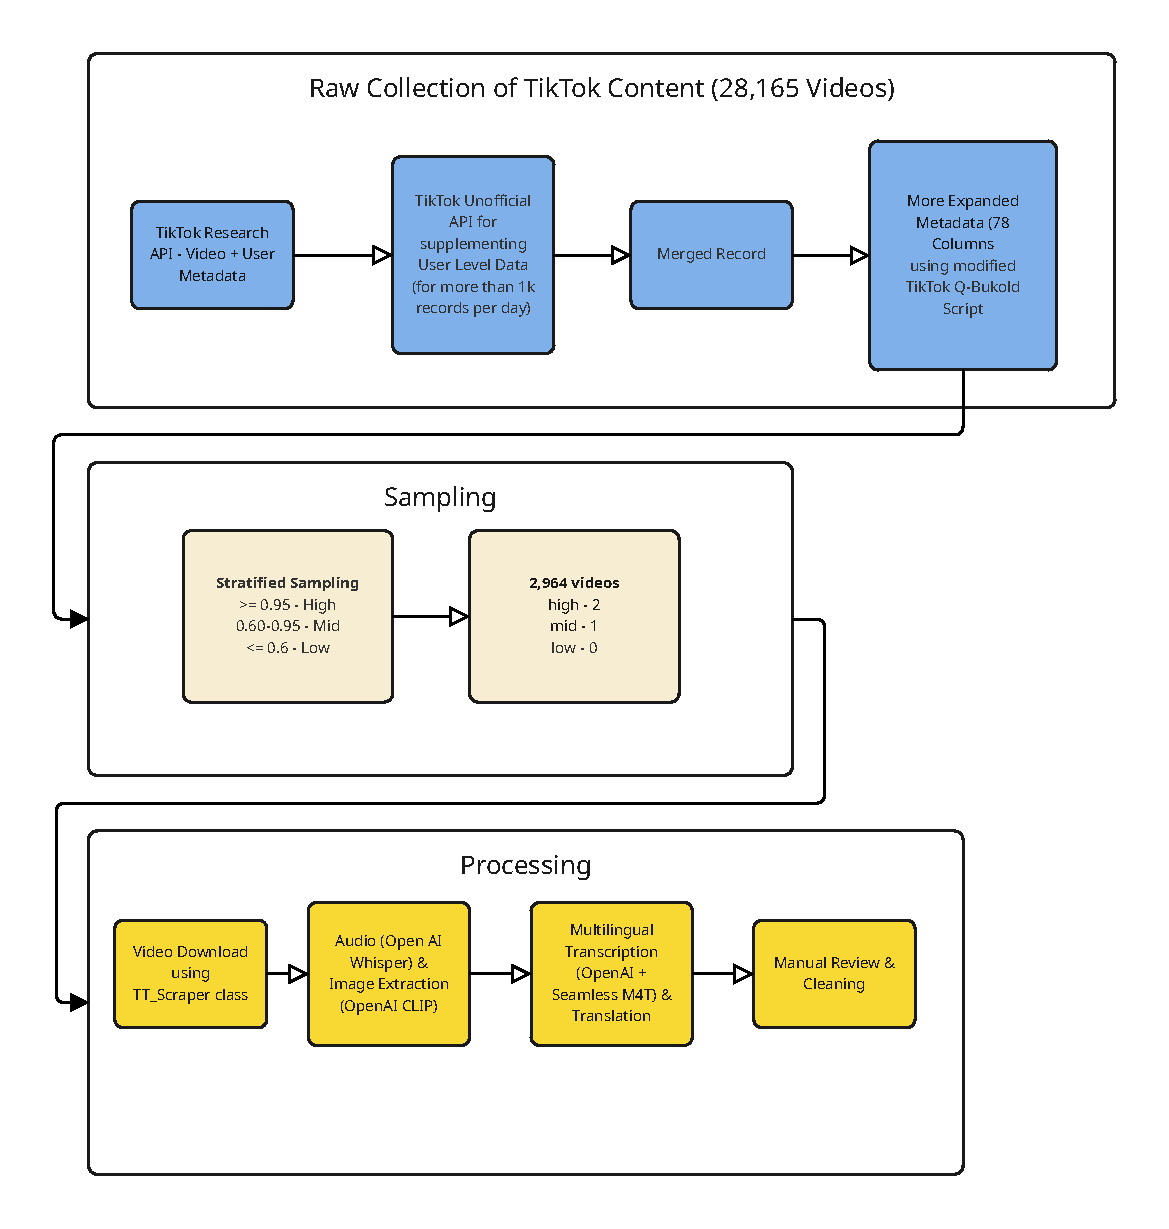
\includegraphics[width=0.6\textwidth, page=1]{figures/data_collection.pdf}
    \caption{Data Collection Pipeline}
    \label{fig:data_pipeline}
\end{figure}
\begin{figure}[H]
    \centering
    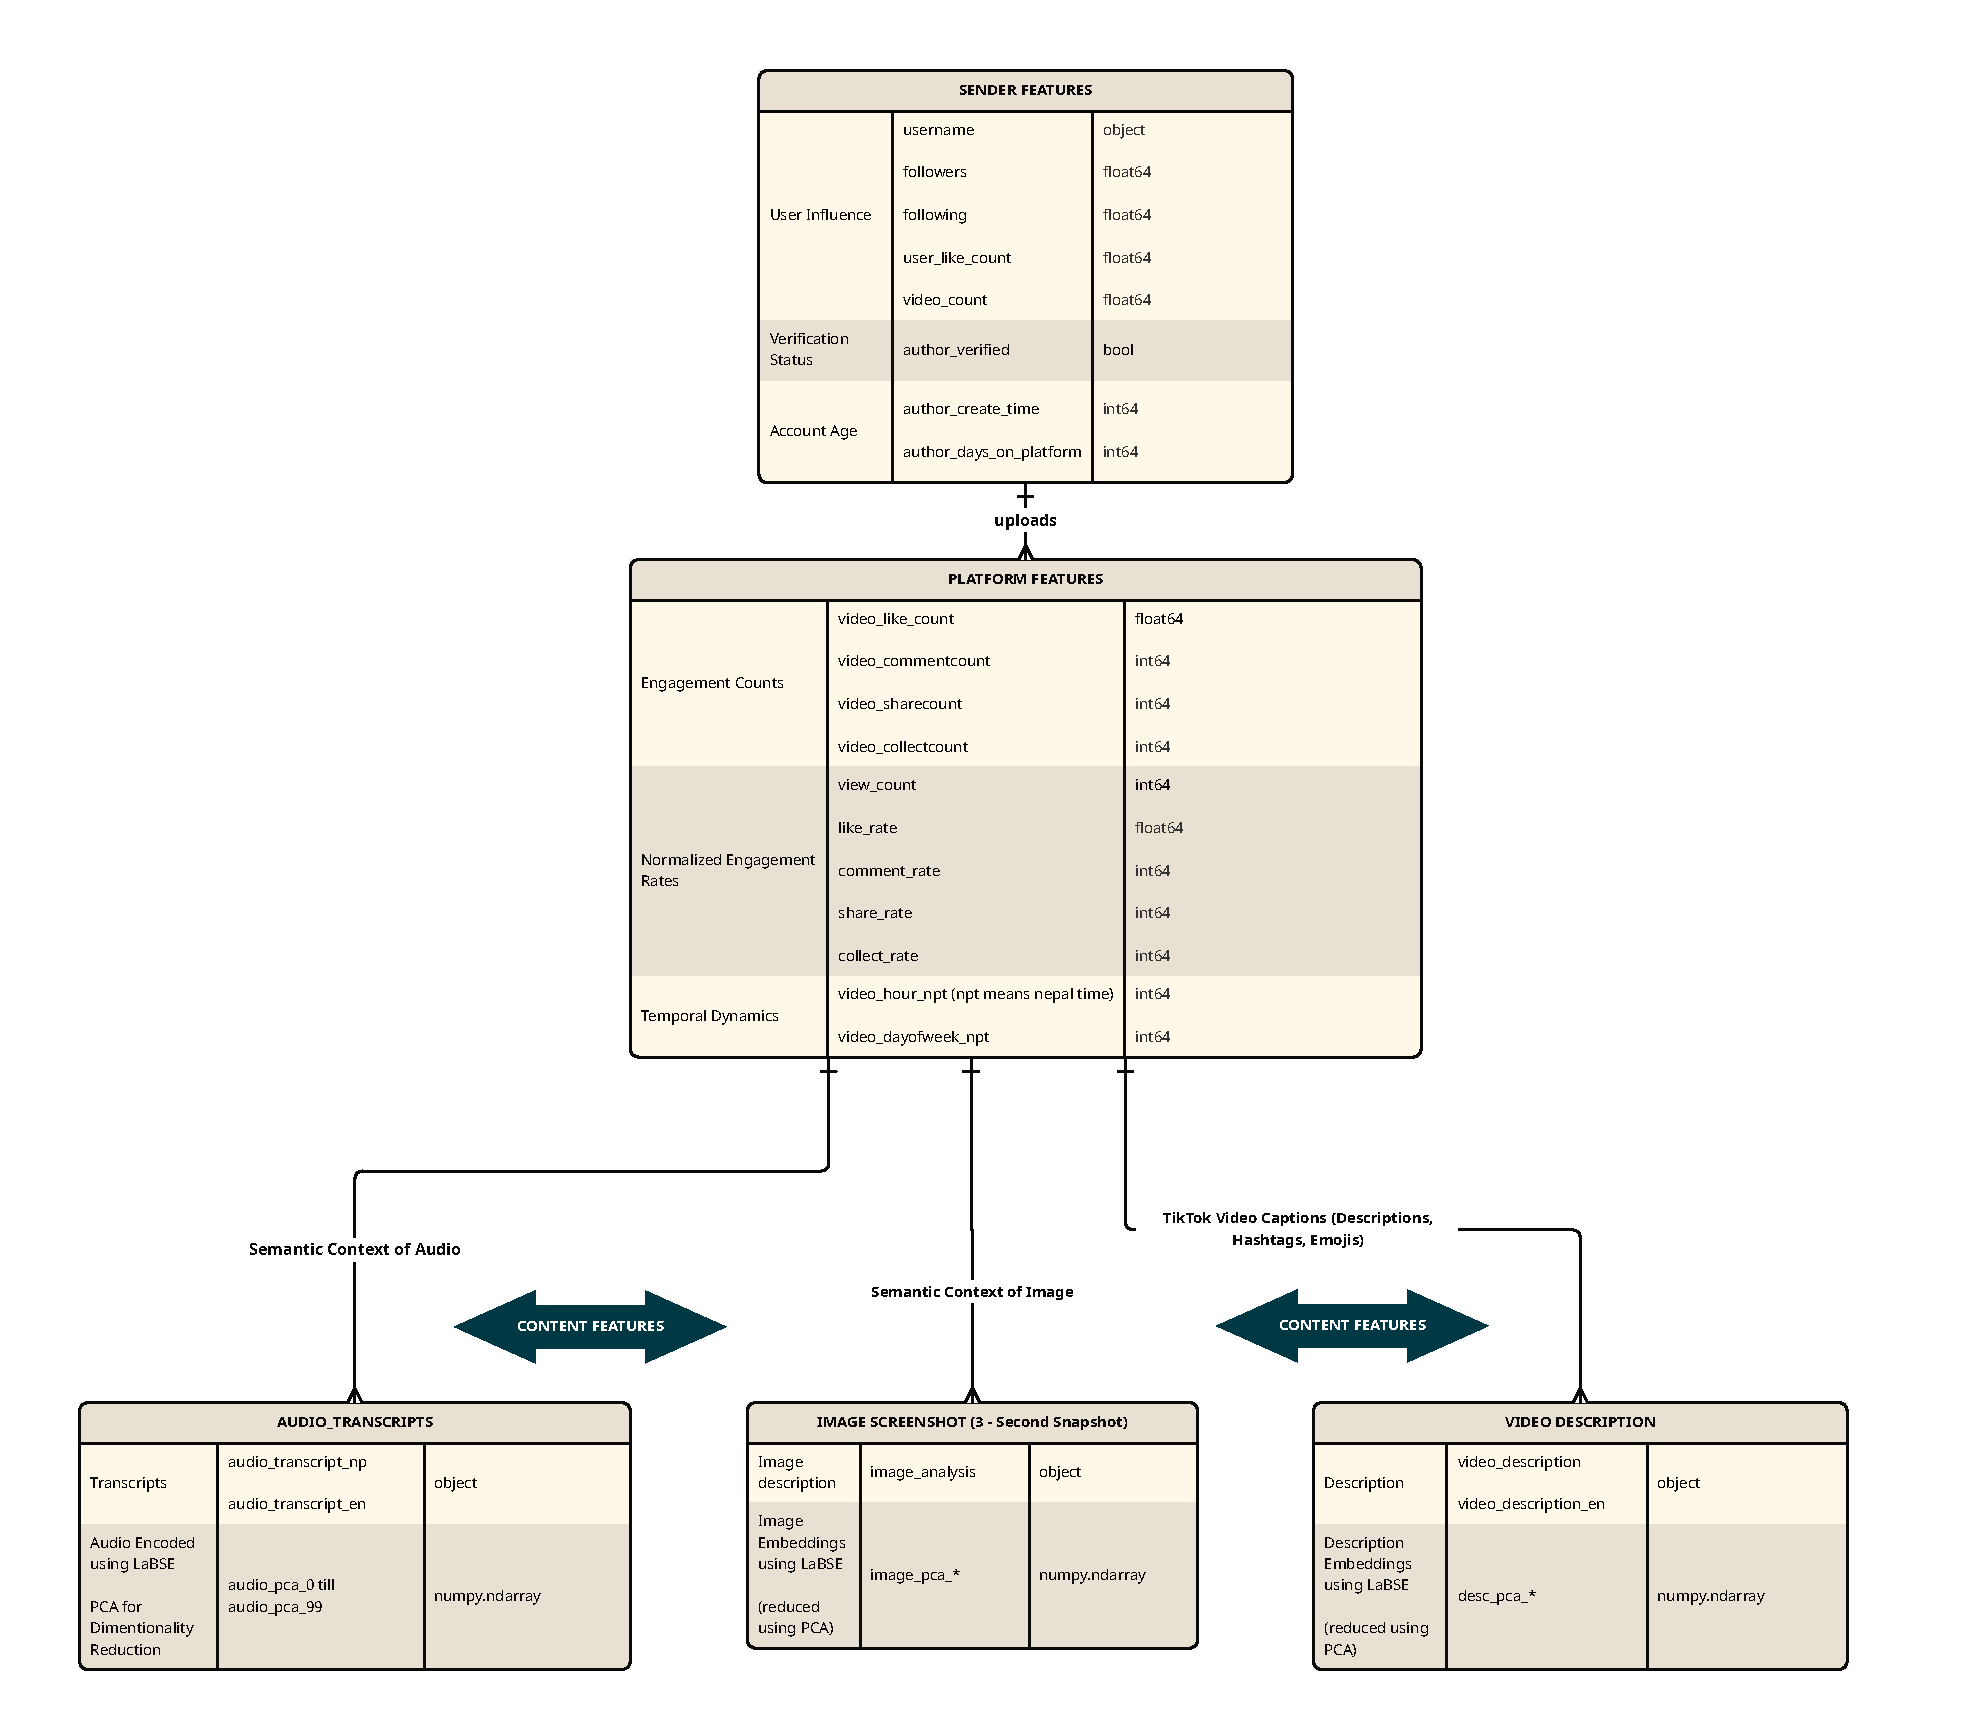
\includegraphics[width=1.0\textwidth, page=1]{figures/data_collection_schema.pdf}
    \caption{Data Schema Collection}
    \label{fig:data_schema}
\end{figure}
\newpage
\section{Feature Engineering}
\subsection{Operationalizing Virality (Dependent Variable)}
No universally accepted standard measure for predicting virality on TikTok was found on my literature, however several research projects and commercial tools have proposed their own metrics and predictive models \parencite{roring2024decoding, SahJordan2025DecodingReddit}. Additionally, no prior research had practiced standard virality criteria of TikTok videos in an election setting in Nepal, necessitating a flexible approach to capture its role in driving public attention during Nepal’s 2022 elections. For this study, Virality was operationalized as a composite score reflecting relative audience engagement, emphasizing interaction over raw popularity. To do this, four \textbf{normalized engagement rates}.

The rates were combined with the logarithm of raw view count to form a \textbf{virality score}, using a weighted formula that emphasizes active user engagement. The final formula is:
\begin{multline}
\text{virality score} = 0.35 \cdot \log(1 + \text{views}) + 0.25 \cdot \log(1 + \text{like rate}) + 0.20 \cdot \\ \log(1 + \text{comment rate}) + 0.15 \cdot \log(1 + \text{share rate}) \\ + 0.05 \cdot \log(1 + \text{collect rate})
\end{multline}
Weightings of (0.35, 0.25, 0.20, 0.15, 0.05) were assigned to prioritize active engagement behaviors. To assess the robustness of this approach, a sensitivity analysis was conducted using equal weighting across components. The resulting agreement between the original and equal-weight virality labels was 99.53\%, suggesting strong stability of the classification. Given the exploratory nature of this study and time constraints, weightings were fine-tuned iteratively based on observed distributions without external validation.
The score was transformed into a ternary classification label for RQ1:
\begin{itemize}
    \item \textbf{Low Virality (0)}: Bottom third of scores.
    \item \textbf{Moderate Virality (1)}: Middle third.
    \item \textbf{High Virality (2)}: Top third.
\end{itemize}
For RQ2, a log-transformed version of the virality score was used as a continuous regression target to account for its skewed distribution.
\newpage
\section{Multimodal Feature Extraction}

This study extracted multimodal features from a stratified sample of 2,964 TikTok videos to predict virality. Features were derived from three primary modalities: audio transcripts, video descriptions, and visual frames.

\subsection{Textual Features}
Textual or Content features aim to capture the semantic, emotional, and contextual characteristics of a video’s actual media content. These include both linguistic and visual elements:

\subsubsection{Audio Transcripts}

\begin{itemize}
    \item Transcribed using OpenAI’s GPT-4o Whisper API \parencite{OpenAI2024gpt4o}, primarily in Nepali with minor instances of Hindi, Bhojpuri/Maithili, Urdu, and English. Manual corrections added contextual annotations (e.g., \texttt{\{\{Party\_Name\}\} Song}). Transcripts were embedded using the BGE-m3 model \parencite{bge-m3} and reduced via PCA (\texttt{audio\_pca\_0} to \texttt{audio\_pca\_99}).
\end{itemize}

\subsubsection{Video Descriptions}

\begin{itemize}
    \item \textbf{Video Descriptions}: Language detection via LangDetect \parencite{langdetect} identified 494 English and 2,470 non-English (Romanized Nepali-English, Devanagari) descriptions. Non-English descriptions were translated to English using GPT-4o \parencite{OpenAI2024gpt4o}, preserving hashtags and mentions. Descriptions were embedded with BGE-m3 and reduced via PCA (\texttt{desc\_pca\_*}).

    \begin{verbatim}
    prompt = f"Translate the following text to English but keep all 
    hashtags and mentions (like #nepal, @username) 
    unchanged:\n\n{masked_text}"
    \end{verbatim}
\end{itemize}
\newpage
\subsection{Visual Features}
\begin{itemize}
 \item \textbf{Visual Features}: A frame at the 3-second mark was extracted \parencite{TikTokCreative2023}, captioned using GPT-4o Vision API \parencite{OpenAI2024gpt4o}, embedded with BGE-m3, and reduced via PCA (\texttt{image\_pca\_*}).
    \item \textbf{Sentiment Scores}: Extracted for audio, descriptions, and image captions using a pretrained sentiment model.
    \item \textbf{Lexical Features}: Included \texttt{audio\_word\_count}, \texttt{image\_word\_count}, and \texttt{hashtag\_count}.    

\end{itemize}

\subsection{Platform Features}
Platform features refer to platform-mediated affordances and behavioral traces that reflect how users engage with the content:

\begin{itemize}
    \item \textbf{Temporal Dynamics}: \texttt{video\_hour\_npt}, \texttt{video\_dayofweek\_npt}.
    \item \textbf{Metadata}: \texttt{video\_diversification} labels, duet/stitch indicators.
\end{itemize}

\subsection{Sender Features}

Sender features capture the video uploader’s social capital and credibility:

\begin{itemize}
    \item \textbf{Creator Tier Metrics}: A categorical feature, \texttt{creator\_tier}, was derived from follower counts to analyze nonlinear effects of audience reach on virality. Using the empirical distribution of follower counts across 2,964 videos (25th percentile: $\approx 983$, 50th: $\approx 2,191$, 75th: $\approx 8,120$, 90th: $\approx 48,740$, 95th: $\approx 108,700$, 99th: $\approx 376,500$), we defined tiers as: Regular ($< 10,000$ followers), Micro Influencer ($10,000–49,999$), Macro Influencer ($50,000–99,999$), and Mega Influencer ($\geq 100,000$). This data-driven approach ensures relevance to Nepal’s 2022 election context and enhances model interpretability.
\newpage
    \item \textbf{Verification Status}: A binary feature, \texttt{author\_verified}, indicates official TikTok verification, reflecting institutional presence or public figure status that may influence platform distribution and audience trust.
    
    \item \textbf{Account Age}: Derived from \texttt{author\_create\_time}, \texttt{author\_days\_on\_platform} measures the creator’s active duration on TikTok, capturing their tenure and experience, which may affect content strategy and reach.
\end{itemize}
\newpage
\subsection{Feature Integration \& Pre-Processing}

Predictor variables from platform metadata, sender attributes, and content modalities were integrated into a unified, model-ready dataset. Numerical features (e.g., follower count, interaction rates like \texttt{like\_rate}, \texttt{comment\_rate}) were z-score normalized for comparability, while categorical variables (e.g., day-of-week) were one-hot encoded. Multimodal embeddings from audio transcripts, image snapshots, and video descriptions were generated using a multilingual transformer model, reduced via PCA, and used in their compact latent form without further scaling, as they already captured normalized semantic similarity.

To prevent label leakage, post-performance variables (\texttt{video\_like\_count}, \texttt{video\_commentcount}, \texttt{video\_sharecount}, and their normalized counterparts \texttt{like\_rate}, \texttt{comment\_rate}, \texttt{share\_rate}, \texttt{collect\_rate}) were excluded, focusing strictly on pre-upload features like content semantics (text, image, audio) and user metadata (e.g., \texttt{creator\_tier}, verification status). This structured predictor matrix ensured consistent model input and enabled nuanced evaluation of content, platform, and sender contributions to virality prediction.

\section{Sentence Embedding Model Selection}
We evaluate four sentence embedding models on Nepali election-related texts:
\begin{itemize}
    \item LaBSE \parencite{reimers-2019}
    \item paraphrase-multilingual-MiniLM-L12-v2 (MiniLM-L12) \parencite{paraphrase-multilingual-MiniLM-L12-v2}
    \item all-MiniLM-L6-v2 \parencite{all-MiniLM-L6-v2}
    \item BGE-M3 \parencite{bge-m3}
\end{itemize}

BGE-M3 demonstrates multi-lingual capabilities supporting 100+ languages with dense/sparse retrieval \parencite{bge-m3}. The MiniLM variants offer optimized performance for semantic similarity tasks \parencite{reimers-2019}.

Based on evaluation of sentence-embeddings (See Table~\ref{tab:embedding_comparison_appendix}) for 11-pairs of random sentence-text pairs, BGE-m3 was chosen for its more balanced performance in compared to other models. 

\section{Analytical Framework}

The analysis addresses the two research questions through two complementary approaches:

\subsection{Machine Learning for Virality Prediction (RQ1)}
\begin{itemize}
    \item \textbf{Model, Training, and Validation}: XGBoost was selected as the primary classifier over Random Forest and LightGBM (see Section~\ref{sec:model_selection}). The stratified sample of 2,964 videos was split into 70\% training and 30\% test sets, evaluated using accuracy, precision, recall, F1-score, and AUC-ROC.
    
    \item \textbf{Explainability and Error Analysis}: SHAP (SHapley Additive Explanations) was applied to XGBoost to interpret feature contributions, where predictions are decomposed as $f(x) = \text{base value} + \sum \text{SHAP values}$, focusing on metadata (e.g., \texttt{user\_like\_count}, \texttt{author\_days\_on\_platform}), visual/audio embeddings (e.g., \texttt{image\_pca\_*}, \texttt{audio\_pca\_*}), and descriptive text features (e.g., \texttt{desc\_pca\_*}, \texttt{sentiment scores}). Potential biases were assessed through qualitative error analysis of misclassified samples.
\end{itemize}

\subsection{Content Analysis for Communication Styles and Political Affiliations (RQ2)}
\begin{itemize}
    \item \textbf{Communication Styles}: Videos were annotated with a revised codebook adapted from \parencite{schellewald2021communicative, umansky2023dances}, categorizing 11 styles, with added Nepal-specific categories (e.g., Entertainment/Song, Charismatic/Leadership Appeal) to reflect cultural context and independent voices \parencite{DW2022NepalElections} (see Appendix~\ref{app:codebook}). Each video received a primary (\texttt{Style\_1}) and secondary (\texttt{Style\_2}) style, but \texttt{Style\_2} was excluded due to limited coverage (40\%) and time constraints.
    
    \item \textbf{Political Affiliations and Annotation}: Audio transcripts were categorized into 17 themes (e.g., campaign songs, comedic sketches) via GPT-4o zero-shot classification, then filtered into four Nepal 2022 election categories: \textit{Nepali Congress}, \textit{UML}, \textit{Maoist}, and \textit{Independent}. Labels were verified using multimodal cues (party symbols, candidate names, slogans, election songs, visuals).
    
    \item \textbf{Regression Modeling and Visualization}: OLS regression analyzed the effect of styles and affiliations on log-transformed, z-scored virality, using \textit{Civic Awareness} as the reference style and \textit{general election content} as the baseline theme, with dummy-encoded variables, assumed homoscedasticity, and 95\% confidence intervals. A heatmap visualized mean z-virality-scores across style–theme pairs.
\end{itemize}

\section{Data Annotation and Validation}
\label{sec:data_annotation}

A systematic annotation and validation process ensured the robustness of multimodal features and labels for the XGBoost model (RQ1) and OLS regression (RQ2) using 2,964 TikTok videos from Nepal’s 2022 elections.

\subsection{Audio Transcripts}
A 5\% sample (\(n=148\)) of Nepali audio transcripts (\texttt{audio\_transcript\_np}), converted to PCA embeddings (\texttt{audio\_pca\_*}), was manually validated, achieving 87.2\% accuracy by the primary author and a Cohen’s Kappa of 0.462 (moderate agreement) with a secondary evaluator \parencite{landis1977measurement}. Despite dialectal challenges, embeddings were retained due to their complementary role with image (\texttt{image\_pca\_*}) and description (\texttt{desc\_pca\_*}) embeddings, with \texttt{audio\_pca\_0} showing a mean $|$SHAP$|$ $\approx$ 0.3.

\subsection{Video Descriptions}
A 5\% sample (\(n=148\)) of translated video descriptions achieved 98.6\% accuracy, preserving hashtags per best practices \parencite{highfield2016instagrammatics}. These were converted to PCA embeddings (\texttt{desc\_pca\_*}) for the XGBoost model.

\subsection{Image Embeddings}
Image embeddings (\texttt{image\_pca\_*}) were generated using OpenAI’s CLIP API \parencite{radford2021learning}, recognized for high accuracy, and directly used in the XGBoost model without manual validation, with \texttt{image\_pca\_2} showing a mean $|$SHAP$|$ $\approx$ 0.1 for high-virality predictions.

\subsection{Style and Content Labels for RQ2}
Three annotators labeled all 2,964 videos for communication styles (\texttt{style\_1\_label}, e.g., Comedic) and content themes (\texttt{content\_label}, e.g., party affiliation) per a predefined codebook. A 150-video sample yielded a Cohen’s Kappa of 0.622 (substantial agreement) for \texttt{style\_1\_label} \parencite{landis1977measurement}, supporting its use in OLS regression. Content labels, derived via zero-shot classification and manually reviewed, lacked formal validation due to resource constraints.

\subsection{Discussion}
Validation confirms reliability, with 98.6\% accuracy for video descriptions and Kappa = 0.622 for style labels, though audio transcripts’ Kappa = 0.462 reflects linguistic challenges. CLIP embeddings align with computer vision standards, and zero-shot content labels were mitigated by manual review. This ensures dataset suitability for modeling virality and style–theme interactions, though future work could improve audio transcription using advanced multilingual NLP fine-tuned for Nepalese social media communication context.

\section{Ethical Considerations}
Data collection complied with TikTok’s privacy policies. No PII was collected. Approval was obtained from the Hertie Data Science Review Board. Dataset limitations and potential biases were transparently reported.


\chapter{Results}
\section{Exploratory Analysis}
Exploratory Analysis was conducted on the full dataset. For Dataset summary (see Table~\ref{tab:dataset_summary})

\subsection{Number of Videos Over Time}
Figure~\ref{fig:tiktok_video_post} illustrates the volume of TikTok videos posted over this time frame. A noticeable rise in content production is observed as the election approaches, peaking sharply on Election Day (May 13, 2022).

\begin{figure}[htbp]
    \centering
    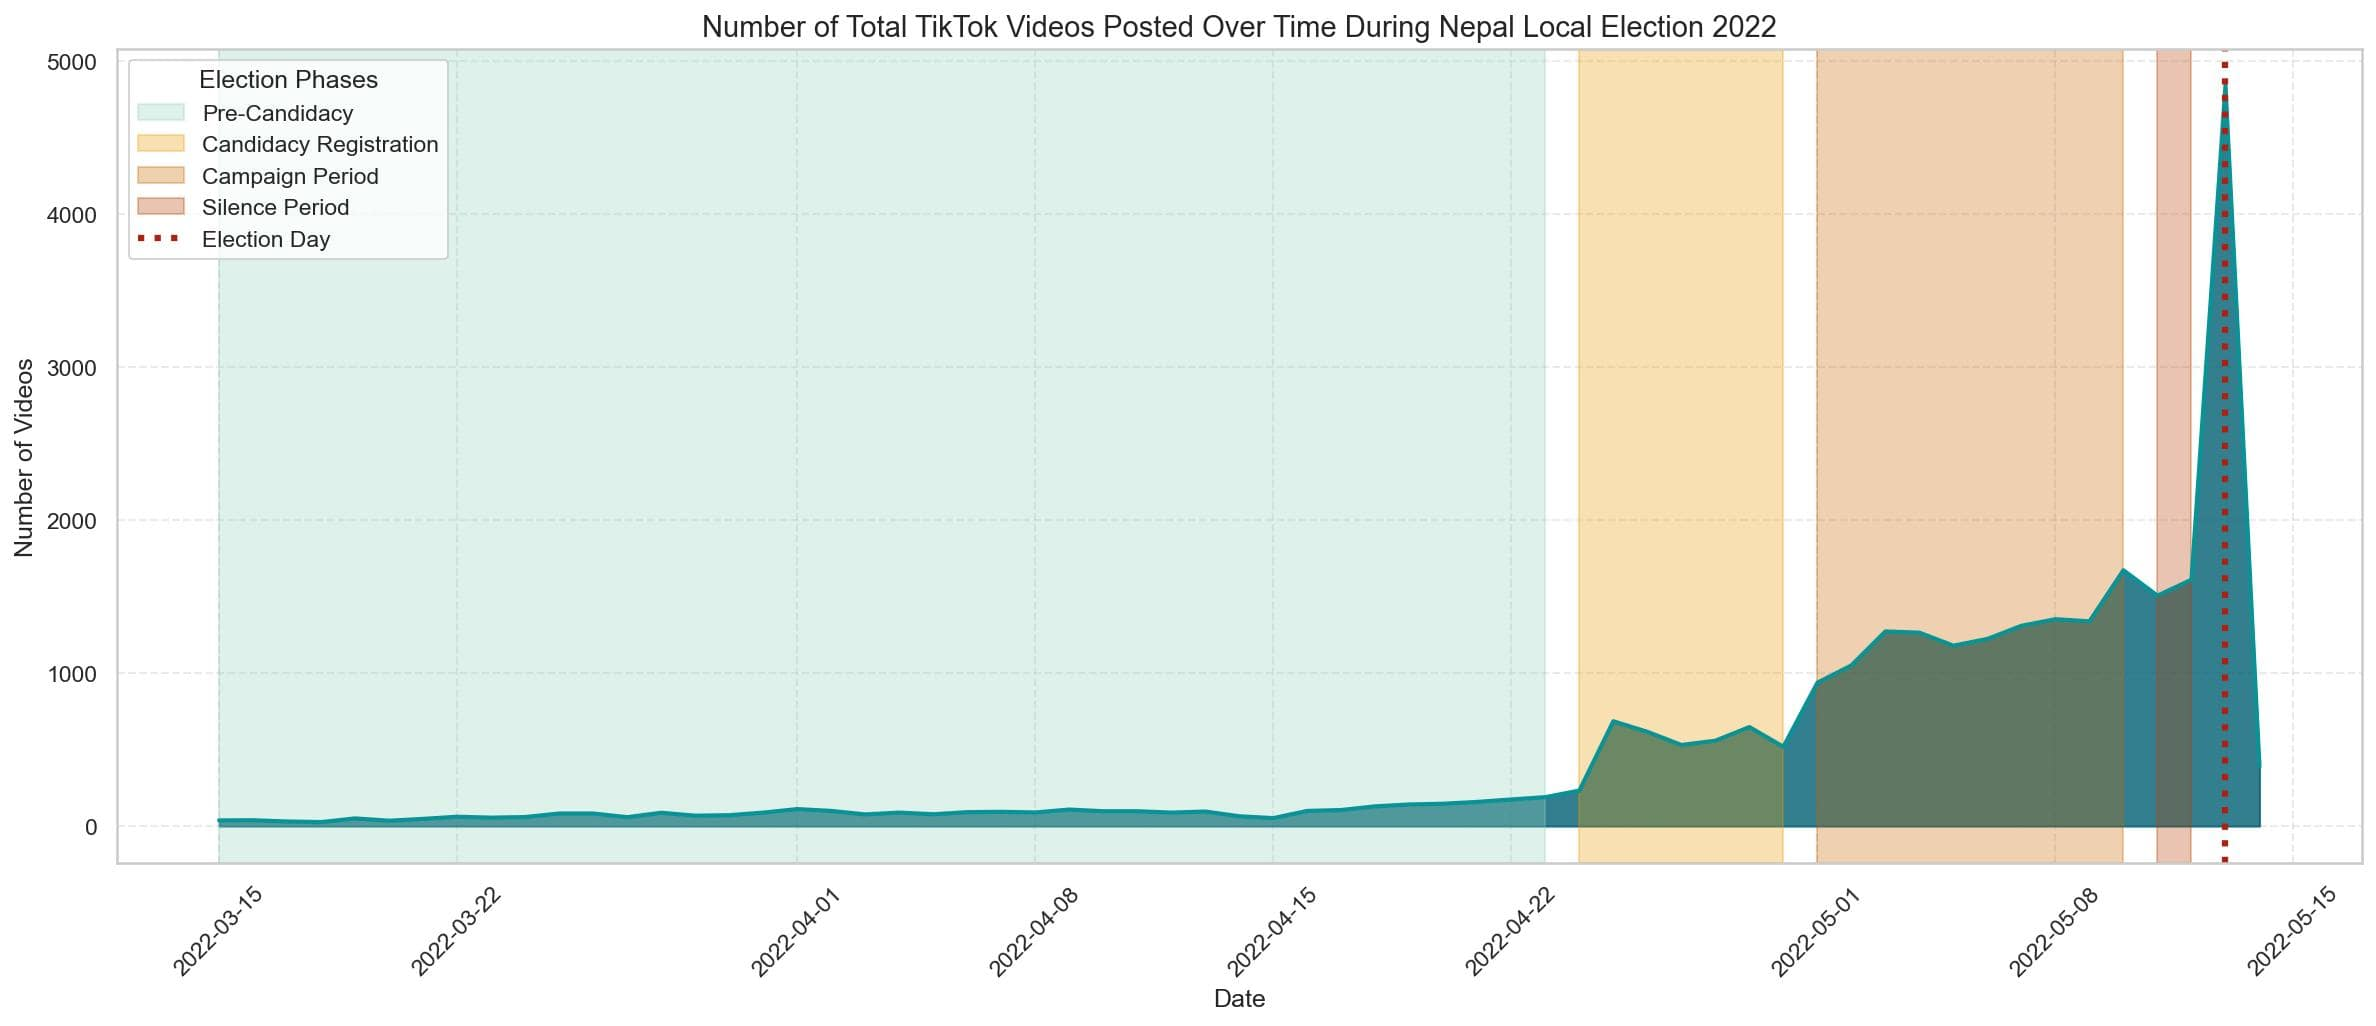
\includegraphics[width=0.99\textwidth]{figures/EDA/tiktok_video_counts_election_period.jpg}
    \caption{TikTok Video Post Over Time)}
    \label{fig:tiktok_video_post}
\end{figure}
\newpage
\subsection{Post Volume Heat Map}

Figure~\ref{fig:tiktok_heatmap_postcount} reveals that most video posts occur on Fridays, particularly during the late afternoon and evening hours. A distinct posting peak is observed at 21:00 (9:00 PM NPT), suggesting that content creators might be strategically timing their posts to maximize visibility and engagement during the end of their weekdays. 

\begin{figure}[htbp]
    \centering
    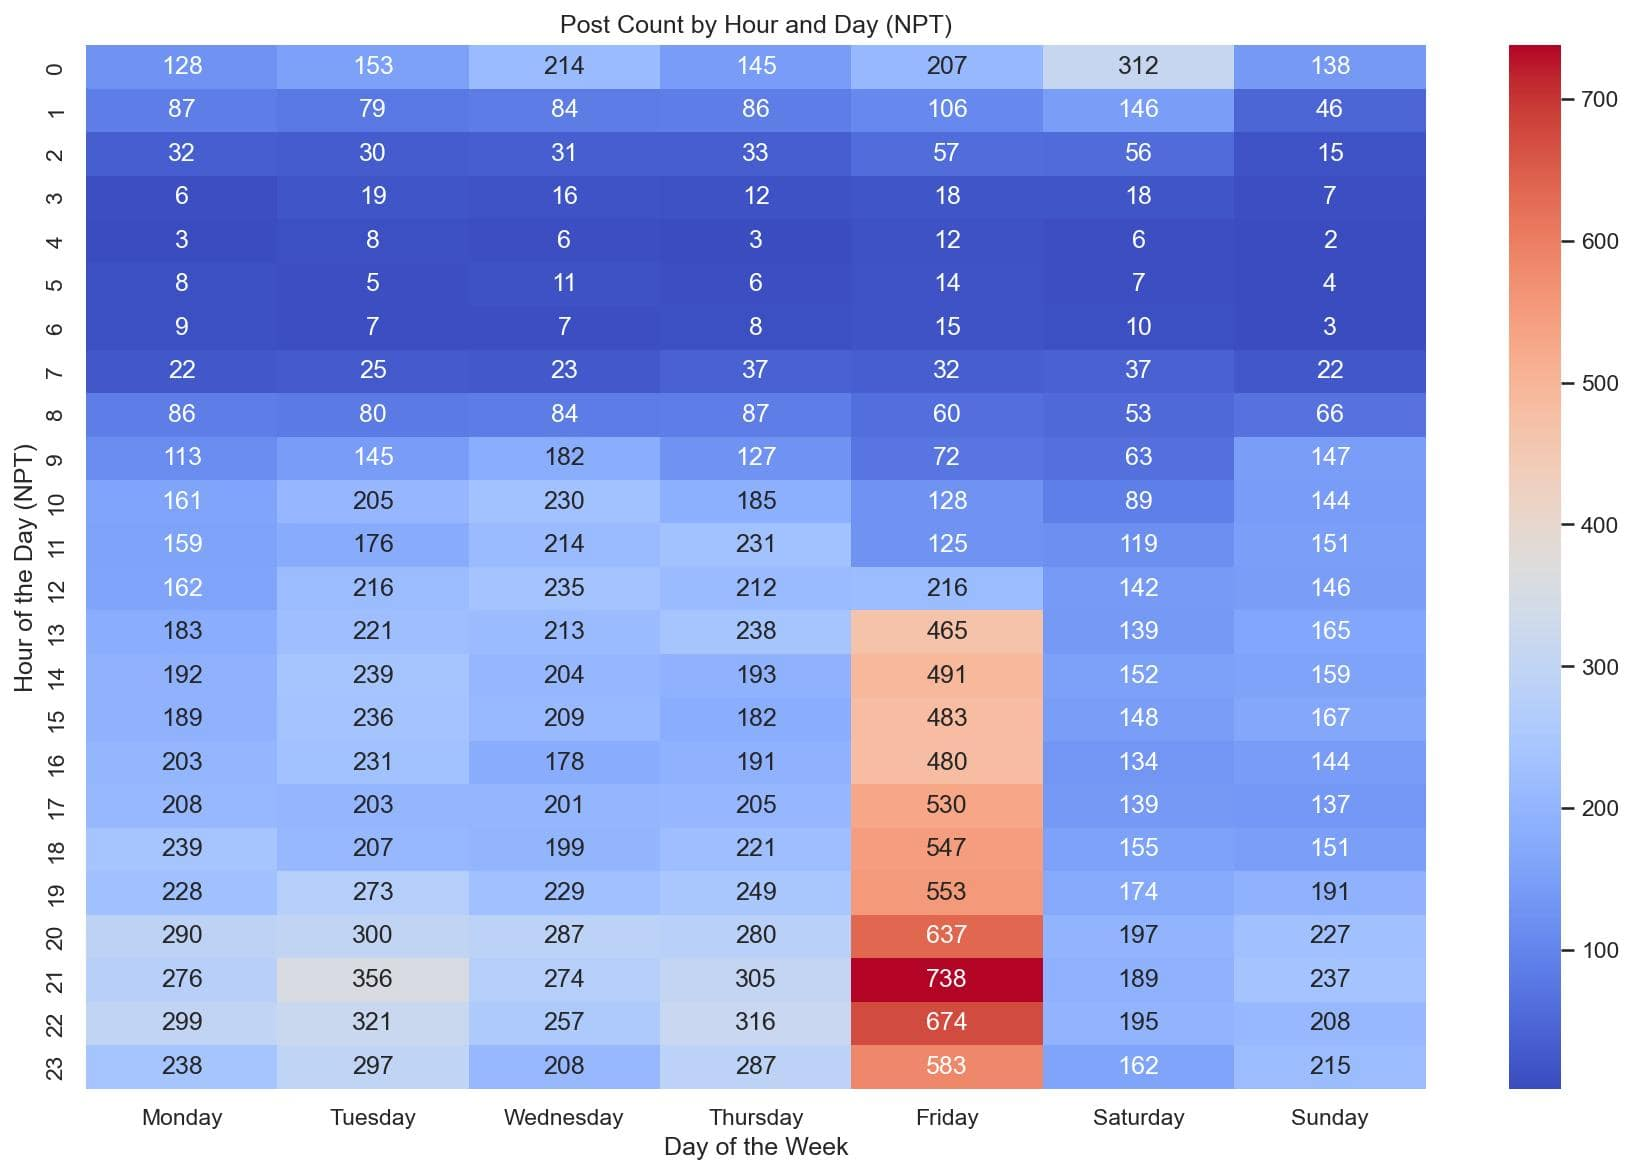
\includegraphics[width=0.60\textwidth]{figures/EDA/heatmap_post_count.jpg}
    \caption{TikTok Video Post Over Time)}
    \label{fig:tiktok_heatmap_postcount}
\end{figure}


\subsection{Top Keywords in Video Descriptions}

The dataset includes 20,237 unique hashtags extracted from video descriptions. 

After applying a custom stopword filter to remove generic or repetitive terms (e.g., \texttt{fyp, viral, trending}), we generated a word cloud to visualize prominent hashtags. Figure~\ref{fig:wordcloud} reveals Nepali keywords like \textit{chunab} ("election") and \textit{chunablagyo} ("election vibes"), as well as direct references to political campaigns. Note that some Devanagari (Nepali) script tokens are rendered as square boxes due to font encoding limitations.

Furthermore,Table~\ref{fig:top_political_hashtag} lists the 20 most frequently occurring hashtags in the political genre along with their respective counts.

\begin{figure}[htbp]
    \centering
    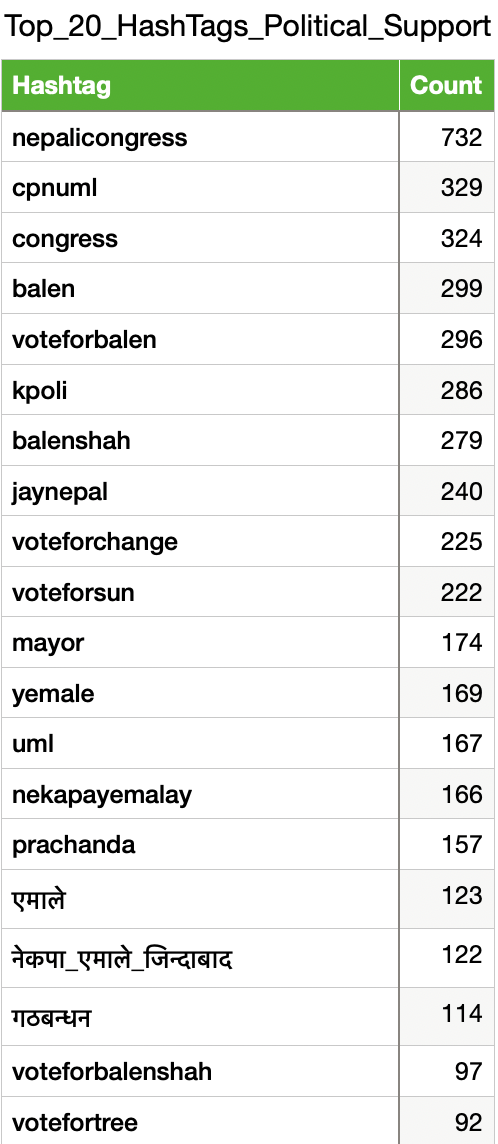
\includegraphics[width=0.30\textwidth]{figures/EDA/Top_20_Political_Hashtag.png}
    \caption{Top Political Hashtags Used During Local Election 2022}
    \label{fig:top_political_hashtag}
\end{figure}

\begin{figure}[htbp]
\centering
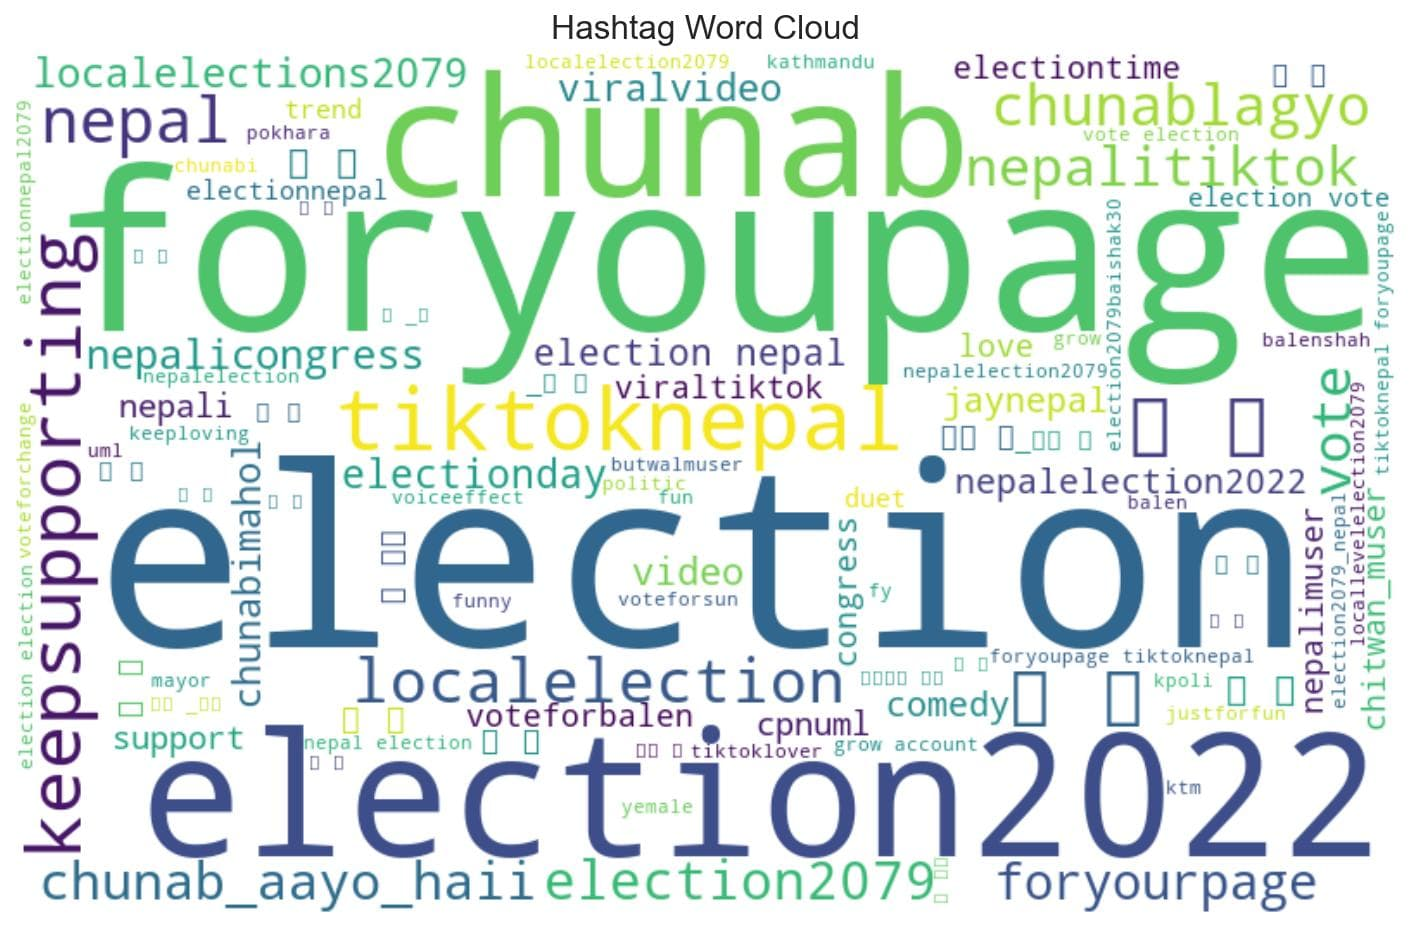
\includegraphics[width=0.60\textwidth]{figures/EDA/wordcloud.jpg}
\caption{Top Filtered hashtags after removing trending terms}
\label{fig:wordcloud}
\end{figure}

% To be filled: Classifier performance, SHAP visualizations, regression coefficients
\clearpage
\section{Virality Prediction Results}
This section presents the results for our first research question, which aimed to study virality prediction using pre-upload content, platform, and sender characteristics. To focus on pre-upload features, post-upload engagement metrics (e.g., views, likes) were excluded. Results are organized into model performance, feature importance, ablation study, error analysis, and explainability using SHAP.


\subsection{Model Performance}
\label{sec:model_selection}
To select an appropriate model for predicting TikTok virality, three algorithms were compared: Random Forest, XGBoost, and LightGBM. These models were trained with default parameters on a stratified train-test split (70\% train, 30\% test, n=890 test samples). Random Forest served as a baseline due to its simplicity, while XGBoost and LightGBM were chosen for their advanced gradient boosting capabilities, suitable for high-dimensional datasets with mixed features (numerical, categorical, embeddings). Performance was evaluated using accuracy, macro average F1-score, and AUC-ROC (one-vs-rest).

Performance metrics included accuracy, macro F1, and class-specific F1 scores for three virality classes: low (0), mid (1), and high (2). The baseline accuracy for random guessing in a three-class problem is 33.33\%.

The comparison (Table \ref{tab:model_performance}) showed that LightGBM achieved the highest accuracy (0.61) and AUC-ROC (0.7972), followed closely by XGBoost (accuracy: 0.60, AUC-ROC: 0.7948), while Random Forest lagged (accuracy: 0.58, AUC-ROC: 0.7526). All models struggled with medium virality (Class 1, F1-scores: 0.48–0.52), but performed well on high virality (Class 2, F1-scores: 0.66–0.68). XGBoost was selected for further optimization due to its competitive performance, suitability with lesser data, robustness to noisy data, and flexibility for hyperparameter tuning (compared to LGB), which offered potential for improvement.

\begin{table}[h]
\centering
\caption{Model Comparison Results (Default Parameters)}
\label{tab:model_performance}
\begin{tabular}{lccc}
\toprule
\textbf{Model} & \textbf{Accuracy} & \textbf{Macro Avg F1-score} & \textbf{AUC-ROC (OvR)} \\
\midrule
Random Forest & 0.58 & 0.58 & 0.7526 \\
XGBoost       & 0.60 & 0.60 & 0.7948 \\
LightGBM      & 0.61 & 0.60 & 0.7972 \\
\bottomrule
\end{tabular}
\end{table}


\subsection{Performance of the Tuned XGBoost Model}
The tuned XGBoost model was evaluated on the test set (n=890), achieving an accuracy of 0.60, a macro average F1-score of 0.60, and an AUC-ROC of 0.7871, slightly below the default LightGBM (AUC-ROC: 0.7972) but comparable to the default XGBoost (AUC-ROC: 0.7948). Detailed performance metrics are presented in Table~\ref{tab:classification_report_xgboost} 

\begin{table}[h]
\centering
\caption{Classification Report for Tuned XGBoost Model}
\label{tab:classification_report_xgboost}
\begin{tabular}{lcccc}
\toprule
\textbf{Class} & \textbf{Precision} & \textbf{Recall} & \textbf{F1-score} & \textbf{Support} \\
\midrule
0 (Low-Viral)     & 0.56 & 0.72 & 0.63 & 294 \\
1 (Mid-Viral)     & 0.53 & 0.49 & 0.51 & 293 \\
2 (High-Viral)    & 0.75 & 0.60 & 0.67 & 303 \\
\midrule
\textbf{Macro Avg}    & 0.61 & 0.60 & 0.60 & 890 \\
\textbf{Weighted Avg} & 0.62 & 0.60 & 0.60 & 890 \\
\bottomrule
\end{tabular}
\end{table}

The tuned model maintained strong performance for low virality (Class 0, F1-score: 0.63) and high virality (Class 2, F1-score: 0.67), with high recall for Class 0 (0.72) and high precision for Class 2 (0.75). However, it continued to struggle with medium virality (Class 1, F1-score: 0.51), consistent with the baseline models, likely due to overlapping feature distributions in this range. The AUC-ROC of 0.7871 indicates robust discriminative ability across classes, though the slight decrease from the default XGBoost suggests that the tuned parameters may have prioritized balance over maximizing AUC-ROC.
\newpage
\section{Feature Importance Analysis}
SHAP (SHapley Additive exPlanations) values were used to assess feature importance, measuring the average impact of each feature on the model’s predictions across the three classes on the full test set (n=890). The top 20 features are shown in the SHAP summary plot (Figure~\ref{fig:shap_summary}), and mean SHAP values for feature groups are presented in Table~\ref{tab:shap_values}

\begin{figure}[h]
    \centering
    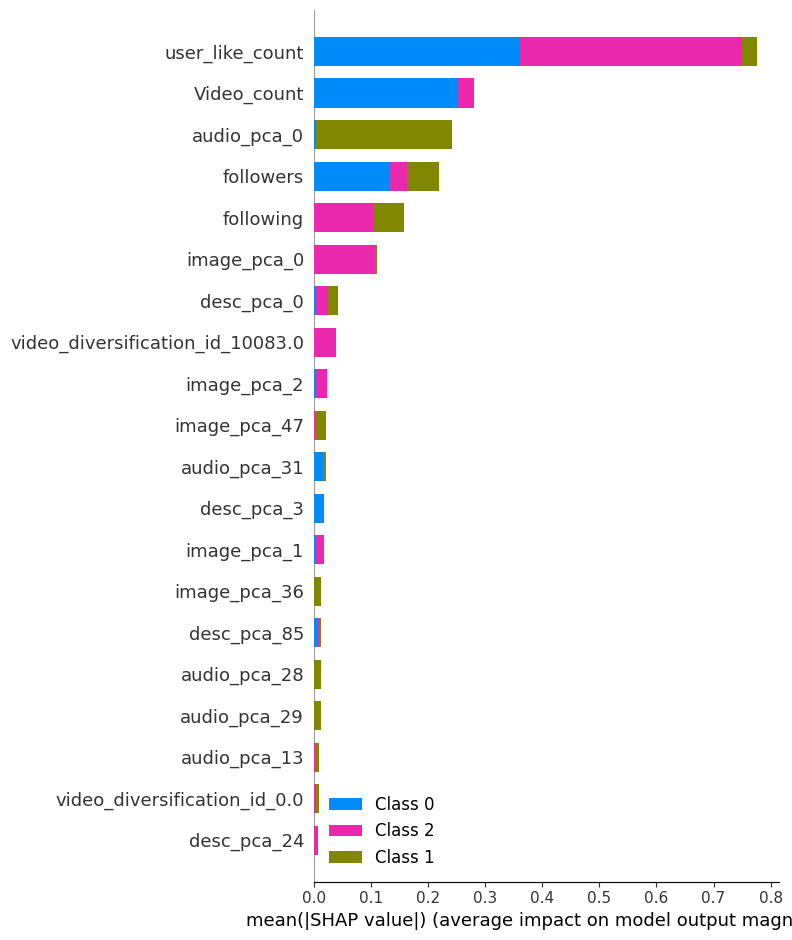
\includegraphics[width=0.60\textwidth]{figures/RQ1/SHAP_first_test_Plot.png}
    \caption{SHAP summary plot of top 20 features impacting virality prediction, with contributions to low (Class 0, blue), medium (Class 1, green), and high (Class 2, pink) virality.}
    \label{fig:shap_summary}
\end{figure}


\begin{table}[h]
    \centering
    \caption{Mean SHAP Values for Feature Groups}
    \label{tab:shap_values}
    \begin{tabular}{l S[table-format=1.4]}
        \toprule
        \textbf{Feature Group} & {\textbf{Mean SHAP Value}} \\
        \midrule
        Audio  & 0.0013 \\
        Image  & 0.0010 \\
        Text   & 0.0007 \\
        Sender & 0.0480 \\
        Platform & 0.0004 \\
        \bottomrule
    \end{tabular}
\end{table}

\subsection{Sender Characteristics (Mean SHAP: 0.0480)}
Sender features were the dominant predictors, with a mean SHAP value of 0.0480.
\begin{itemize}
    \item \texttt{user\_like\_count} (mean $|$SHAP$|$ $\approx$ 0.80): Creators’ total likes strongly predicted high virality (Class 2), reflecting established creators’ influence in Nepal’s 2022 election.
    \item \texttt{video\_count} (mean $|$SHAP$|$ $\approx$ 0.40): Prolific creators’ video counts enhanced algorithmic visibility across all classes.
    \item \texttt{followers} (mean $|$SHAP$|$ $\approx$ 0.3): Follower count and network engagement significantly impacted high virality (Class 2), with a minor effect on low virality (Class 0).
\end{itemize}

\subsection{Content Characteristics}
Content embeddings dominated the top 20 features, though with smaller individual impacts than sender features:
\begin{itemize}
    \item \texttt{audio\_pca\_0} (mean $|$SHAP$|$ $\approx$ 0.35): The first audio PCA component notably impacted medium virality (Class 1), suggesting semantic audio content (e.g., election messages) drove moderate engagement.
    \item \texttt{image\_pca\_0}, \texttt{image\_pca\_1}, \texttt{image\_pca\_2} (mean $|$SHAP$|$ $\approx$ 0.05--0.2): Multiple image PCA components appeared, showing high influence, primarily image\_pca\_0 for Class 2 (high-viral).
    \item \texttt{desc\_pca\_0} (mean $|$SHAP$|$ $\approx$ 0.1), \texttt{desc\_pca\_3} (mean $|$SHAP$|$ $\approx$ 0.05): Text PCA components from video descriptions affected low and high virality (Classes 0 and 2), highlighting captions’ role.
\end{itemize}
Mean SHAP values were low (audio: 0.0013, image: 0.0010, text: 0.0007) due to PCA reduction (100 components per modality). Sentiment scores (\texttt{clean\_audio\_text\_sent\_*}) had minimal impact, likely distributed across embeddings.
\newpage
\subsection{Platform Characteristics (Mean SHAP: 0.0004)}
Platform features had the smallest impact:
\begin{itemize}
    \item \texttt{video\_diversification\_id\_10083.0} (mean $|$SHAP$|$ $\approx$ 0.1): The presence of this diversification ID in the top 10 suggests its moderate association with high virality (Class 2). Although its label was missing from the API (see Table~\ref{tab:diversification_label} for details on diversification IDs and their labels), manual inspection of 30 random videos revealed themes often tied to critical speeches, public debates, and civic awareness during the election, with occasional humor and political satire, aligning with the communication styles in Table~\ref{tab:comm_styles_10083}. The missing label reflects data quality issues noted in the Limitations~\ref{limitation}, such as incomplete video metadata.
    \item \texttt{video\_diversification\_id\_0.0} (mean $|$SHAP$|$ $\approx$ 0.05): The default category (2,274 instances) had a minor effect, mainly for low virality (Class 0).
\end{itemize}
The limited impact of platform features may be attributed to challenges in video description processing, such as empty descriptions or misclassification errors, as discussed in the Limitations section.


\begin{table}[h]
    \centering
    \caption{Top Communication Styles for \texttt{video\_diversification\_id = 10083.0}}
    \label{tab:comm_styles_10083}
    \begin{tabular}{l c}
        \toprule
        \textbf{Style} & \textbf{Count} \\
        \midrule
        Critique/Frustration & 103 \\
        Event Coverage & 59 \\
        Civic Awareness & 37 \\
        Comedic & 28 \\
        Charisma/Leadership & 19 \\
        Musical/Entertainment & 14 \\
        Interactive & 7 \\
        Communal & 6 \\
        Personal Vlog/Family & 4 \\
        \bottomrule
    \end{tabular}
\end{table}
\newpage
\subsection{Local Explanation of a High-Virality Prediction}
A local explanation using a SHAP force plot was conducted for a test sample (index 88, $n=890$, video ID: 7093702566613110043) correctly predicted as high-viral (Class 2) by the tuned XGBoost model. The plot (Figure~\ref{fig:shap_force_plot}) shows feature contributions to the Class 2 prediction, starting from a base log-odds of 0.50 and reaching a final prediction value of 0.71.

\begin{figure}[h]
    \centering
    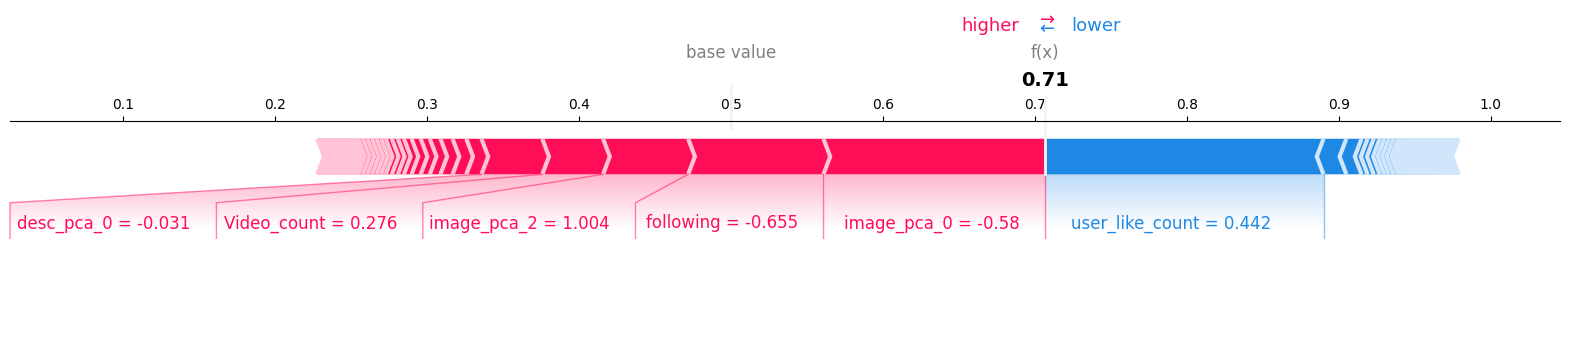
\includegraphics[width=\linewidth]{figures/RQ1/shap_force_plot.png}
    \caption{SHAP force plot for video ID 7093702566613110043, showing feature contributions to high-virality (Class 2) prediction.}
    \label{fig:shap_force_plot}
\end{figure}

\textbf{Positive Contributions (Toward Class 2):}
\begin{itemize}
    \item \texttt{Video\_count} = 0.276 (SHAP: +0.276): The creator’s high video count strongly favored high virality (mean $|$SHAP$|$ $\approx$ 0.5).
    \item \texttt{image\_pca\_2} = 1.004 (SHAP: +1.004): The second image PCA component, tied to visual elements (e.g., news broadcast with airplane inset), boosted the prediction.
    \item \texttt{user\_like\_count} = 0.442 (SHAP: +0.442): The creator’s total likes reinforced high virality (mean $|$SHAP$|$ $\approx$ 0.8).
\end{itemize}

\textbf{Negative Contributions (Against Class 2):}
\begin{itemize}
    \item \texttt{desc\_pca\_0} = -0.031 (SHAP: -0.031): The video description’s first PCA component (e.g., hashtags like \#Localelections2079) slightly reduced virality likelihood.
    \item \texttt{following} = -0.655 (SHAP: -0.655): The creator’s smaller following count limited virality (mean $|$SHAP$|$ $\approx$ 0.3).
    \item \texttt{image\_pca\_0} = -0.58 (SHAP: -0.58): The first image PCA component opposed high virality.
\end{itemize}
(see Appendix~\ref{app:samplecase} for more detail about this sample)
\newpage


\newpage
% --- In your Thesis Main Section (e.g., Results or Analysis) ---
\section{Error Analysis}
An error analysis was conducted on a stratified test sample ($n=890$) to identify misclassification patterns in the tuned XGBoost model (accuracy: 0.60, AUC-ROC: 0.7871) for ternary virality classification (0 = low, 1 = medium, 2 = high). Three specific cases and a general pattern of class boundary errors were examined to understand the model’s behavior.

\textbf{Case 1: Overprediction of Medium Virality as High}
A medium-viral video (ID: 7095593756967046426, true label: 1) with 2,501 views, 232 likes, 3,161 followers, a creator \texttt{user\_like\_count} of 19,854, and \texttt{Video\_count} of 155 was mispredicted as high-viral (Class 2). The model’s reliance on \texttt{user\_like\_count} (mean $|$SHAP$|$ $\approx$ 0.8) and \texttt{Video\_count} (mean $|$SHAP$|$ $\approx$ 0.5), which strongly influence high-virality predictions, likely drove this overprediction, as the creator’s high engagement history overshadowed the video’s moderate engagement metrics.

\textbf{Case 2: Underprediction of High Virality as Medium}
A high-viral video (ID: 7089029999780498715, true label: 2) with 2,820,140 views, 161,239 likes, 2,382 comments, 2,423 shares, 49,400 followers, a \texttt{user\_like\_count} of 1,300,000, and \texttt{Video\_count} of 1,876 was mispredicted as medium-viral (Class 1). Despite exceptionally high engagement metrics, the prediction may have been moderated by content features favoring medium virality (e.g., \texttt{audio\_pca\_0}, mean $|$SHAP$|$ $\approx$ 0.3). Although \texttt{user\_like\_count} and \texttt{Video\_count} strongly support high-virality predictions, the model may struggle to capture the combined effect of extreme engagement values, possibly due to the limited impact of content embeddings (mean SHAP: audio 0.0013, image 0.0010).

\textbf{Case 3: Misclassifications Between Adjacent Classes}
Misclassifications were most frequent between adjacent classes, particularly low (Class 0) and medium (Class 1) virality, with 62\% of Class 1 errors misclassified as Class 0 and 48\% of Class 0 errors as Class 1, highlighting the model’s challenge in distinguishing nuanced engagement levels, as evidenced by the low F1-score for Class 1 (0.51).
\newpage
\section{Communication Styles and Political Content Themes}
To investigate how communication styles and political content themes interact to influence the virality of TikTok videos during Nepal’s local elections, we employed an Ordinary Least Squares (OLS) regression model. The dependent variable was the z-transformed Box-Cox virality score (\( z_{bc_{\text{virality}}} \)), with main effects for communication style and political content theme, their interaction (Style \(\times\) Theme), and control variables including log-transformed follower count, author verification status, and days before election day. Full model output is provided in Appendix~\ref{tab:ols_virality_summary}.

\subsection{Model Performance}
The OLS model explained approximately 16\% of the variance in virality (\( R^2 = 0.159 \), Adjusted \( R^2 = 0.129 \)), a reasonable fit given the high behavioral variability in social media data. The model was statistically significant (\( F = 5.256 \), \( p < 0.001 \)), indicating that communication styles, content themes, and their interactions provide meaningful explanatory power for engagement outcomes.

\subsection{Dataset and Category Inclusion}
The filtered dataset from the sample comprised 1,526 TikTok videos, with political content identified through keyword and theme-based labeling. Five political content categories were included in the analysis, also their name along with their election symbol in Nepali script:
\begin{itemize}[noitemsep]
    \item Independent candidates (e.g., Balen Shah \texthindi{लौरो/स्वतन्त्र}) — count: 232
    \item CPN (UML) (\texthindi{सूर्य/एमाले}) — count: 271
    \item Nepali Congress (\texthindi{रुख/काँग्रेस}) — count: 256
    \item CPN (Maoist) (\texthindi{हँसिया हतौडा/माओवादी}) — count: 84
    \item General election-themed content (non-party affiliated) — count: 687
\end{itemize}
\newpage
Non-political categories (e.g., Bhojpuri, Funny, Speech, Patriotic) were excluded from the OLS regression to maintain thematic focus and address class imbalance but were retained for exploratory style distribution analysis to contextualize broader communication strategies. Certain style--theme combinations, such as Comedic--Maoist (\( n = 5 \)), had limited representation, warranting caution in interpreting their coefficients.

\subsection{Main Effects}
The regression (see Appendix~\ref{tab:ols_virality_main}) revealed significant main effects for communication styles and content themes:
\begin{itemize}[noitemsep]
    \item \textbf{Comedic style} (\( \beta = 1.87 \), \( p = 0.003 \)) and \textbf{Civic Awareness style} (\( \beta = 1.19 \), \( p = 0.037 \)) were positively associated with virality.
    \item \textbf{Independent candidate content} exhibited higher virality compared to the baseline election-themed content (\( \beta = 1.06 \), \( p = 0.028 \)), reflecting strong organic engagement.
    \item \textbf{Control variables}: Verified creators (\( \beta = 0.73 \), \( p = 0.031 \)) and larger follower counts (\( \beta_{\text{log(followers)}} = 0.069 \), \( p < 0.001 \)) were positively associated with virality. Posting earlier before election day had a small but significant effect (\( \beta = 0.0051 \), \( p = 0.039 \)).
\end{itemize}

\begin{figure}[ht]
\centering
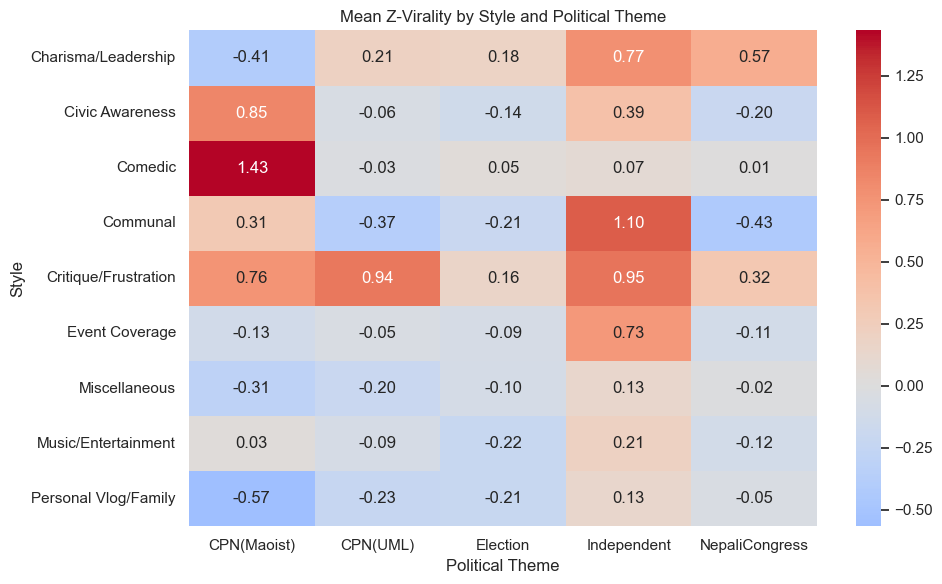
\includegraphics[width=0.8\textwidth]{figures/RQ2/Mean_Z_Virality.png}
\caption{Mean z-transformed virality scores by communication style and political content theme.}
\label{fig:Mean_Z_Virality}
\end{figure}
\newpage
\subsection{Interaction Effects}
Interaction terms highlighted complex dynamics between styles and themes:
\begin{itemize}[noitemsep]
    \item \textbf{Comedic \(\times\) Independent} showed a significant negative interaction (\( \beta = -2.56 \), \( p < 0.001 \)), suggesting that humor, while effective independently, may reduce virality when paired with Independent candidate messaging, possibly due to audience expectations of authenticity or seriousness.
    \item \textbf{Civic Awareness \(\times\) Congress} (\( \beta = -1.94 \), \( p = 0.007 \)) and \textbf{Civic Awareness \(\times\) UML} (\( \beta = -1.47 \), \( p = 0.029 \)) exhibited negative interactions, indicating that educational tones may be less engaging for legacy party content, potentially reflecting skepticism among TikTok’s youth audience.
\end{itemize}

\subsection{Style--Theme Distribution}
Exploratory analysis of style--theme distributions revealed strategic content framing by creators (see Fig.~\ref{fig:TikTokComm}):
\begin{itemize}[noitemsep]
    \item \textbf{Independent candidate content} frequently employed \emph{Charisma/Leadership} (28.4\%) Appeal, often integrating rap or hip-hop (including  form of populism/protest) to blend performance with political branding.
    \item \textbf{Traditional party content} (UML, Congress, Maoist) predominantly used traditional Nepalese-Folk/Traditional styled \emph{Music/Entertainment} (42--48\%) and \emph{Event Coverage}, featuring campaign songs, rallies, and symbolic imagery of their political party like (Tree/ \texthindi{रुख} or green) for support for Congress.
    \item \textbf{Funny content} was overwhelmingly \emph{Comedic or Political Satire} (63.7\%), while \emph{Patriotic} and \emph{Speech} content leaned toward \emph{Civic Awareness} and \emph{Critique/Frustration} - includes discussions involving critic towards government, other political parities, or even among their own party members.
    \item \textbf{Non-political content} (e.g., family vlogs, travel) paired with folk, instrumental, or romantic Nepali pop music, emphasizing cultural and emotional appeal.
\end{itemize}
\textit{Please note the dotted red line indicates the separation between the Political Parties Support/Campaign Songs vs. Other Forms of Audio/Content Theme. }
\begin{figure}[ht]
\centering
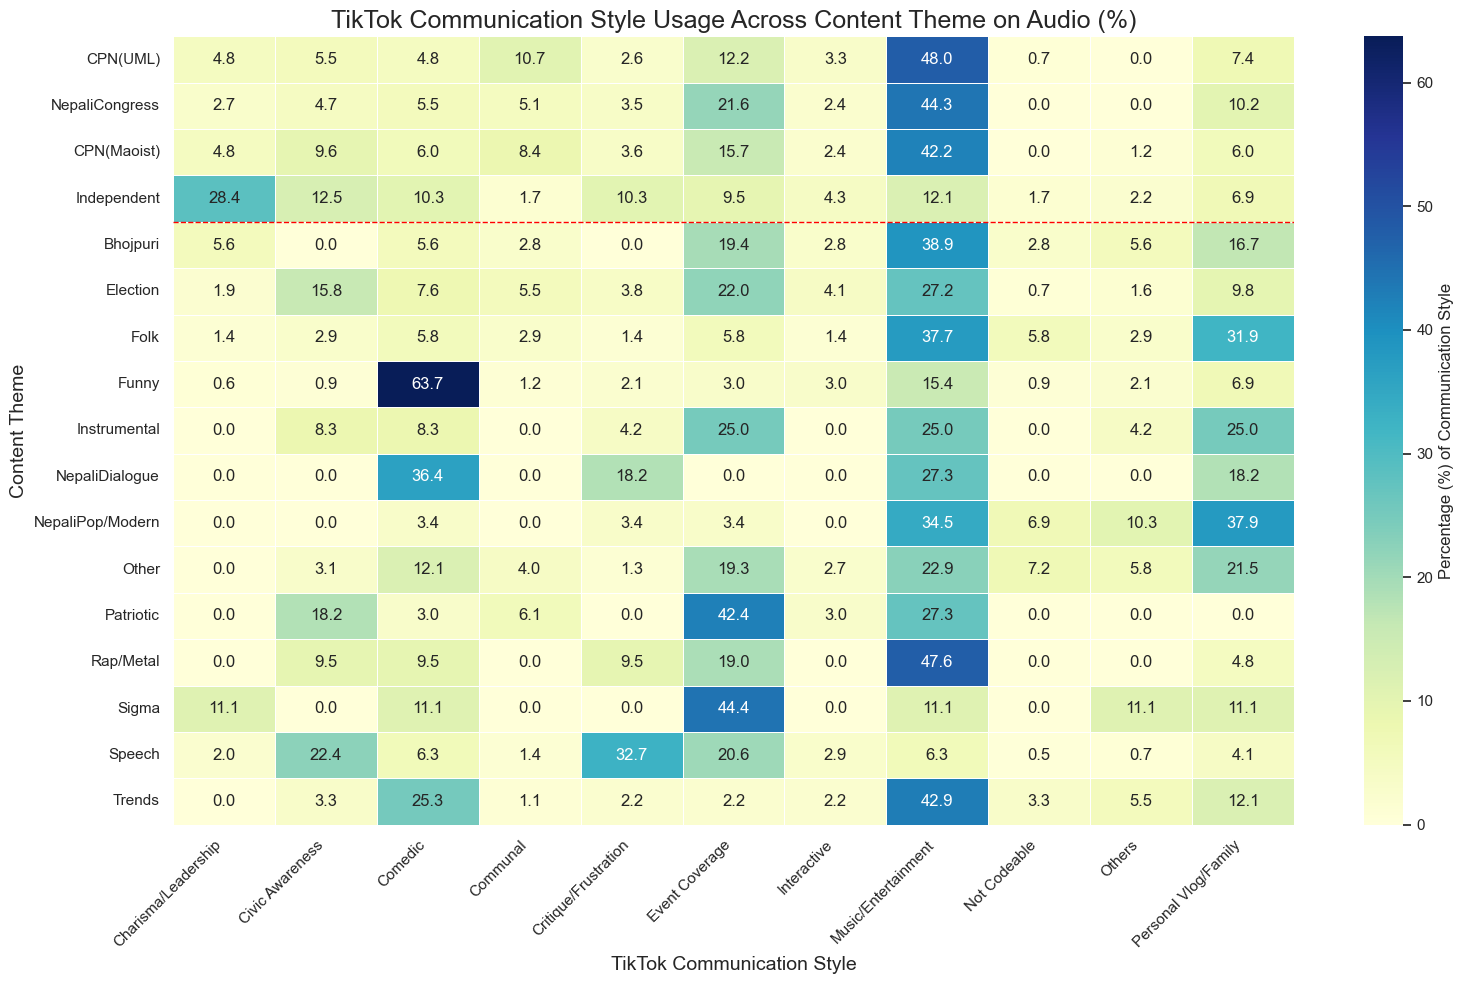
\includegraphics[width=1.0\textwidth]{figures/RQ2/TikTok_Comm_Heatmap.png}
\caption{Heatmap of communication style and content theme distributions.}
\label{fig:TikTokComm}
\end{figure}

\chapter{Discussion}
\label{chap:discussion}

This study examines the predictability of political virality on TikTok during Nepal’s 2022 local election and the interplay of communication styles and political content themes in shaping TikTok engagement (or virality metrics) (RQ2). The findings elucidate the complex dynamics of content, platform, and sender characteristics within a youth-dominated, algorithm-driven social media ecosystem, offering critical insights into digital political communication in a multilingual, politically vibrant context.

\section{Predictability of Political Virality (RQ1)}
\label{sec:rq1_discussion}
The tuned XGBoost classifier achieved an accuracy of 60\%, a macro F1-score of 0.60, and an AUC-ROC of 0.7871, outperforming a random baseline (33.3\%) for the three-class virality prediction task (low, medium, high) on a test set of 890 videos. These results validate the predictive power of pre-upload features—content (audio, image, text embeddings), platform, and sender characteristics.

However, medium virality (Class 1) was challenging, with 62\% of Class 1 errors misclassified as Class 0, reflecting overlapping engagement distributions. Error cases showed biases, such as overprediction for high-profile creators (Case 1, ID: 7095593756967046426) and underprediction for videos with strong engagement but missing comments (Case 2, ID: 7092437819582336283). 

\subsection{Sender Influence and Algorithmic Bias}

Sender characteristics, particularly \texttt{user\_like\_count}, \texttt{Video\_count}, and \texttt{followers} (mean $|\text{SHAP}|$ $\approx$ 0.4), played a significant role in predicting high virality, reflecting TikTok’s bias toward established creators \parencite{bucher2018ifthen}. During Nepal’s 2022 elections, this dynamic amplified the visibility of prominent figures such as independent candidate Balen Shah, whose campaign gained additional momentum through cross-platform promotion, including endorsements from influential pages like Routine of Nepal Banda \parencite{Kandel2024}.
\newpage
Error analysis reveals fairness concerns in virality prediction, as the model’s reliance on sender features like \texttt{user\_like\_count}—mirroring the \texttt{virality\_score} design—often prioritizes established creators (e.g., Case 1 overprediction). This aligns with TikTok’s algorithmic tendency to amplify visible accounts \parencite{noble2018algorithms}, potentially marginalizing grassroots voices and skewing political discourse in Nepal’s election context. However, this also partly explains or contracts with how TikTo's unique affordances also been linked widely with existingl gireuare, how expos-re of low-view vidoes, and its automted "For You" curation, fundamentally reshap or riculatres online, democratizing attengiotn by offering each piece of conent a chance to reach wide aduience\parencite{guinaudeau2022fifteen}. However, The low impact of content embeddings (mean SHAP: audio 0.0013, image 0.0010) suggests PCA reduction limited semantic capture, potentially missing nuanced election themes. 

\subsection{Limits of Predictive Modeling}
The model’s predictive success is tempered by limitations in capturing nuanced social factors, such as cultural authenticity or hyper-local sentiment. The low impact of content embeddings (mean SHAP: audio 0.0013, image 0.0010, text 0.0007) suggests that PCA reduction (100 components) compressed semantic nuances, as seen in the local explanation where \texttt{desc\_pca\_0} negatively impacted prediction. Frequent misclassifications between low and medium virality (62\% of Class 1 errors as Class 0, 48\% of Class 0 as Class 1) reflect overlapping engagement distributions, limiting precision for Class 1. These challenges underscore the difficulty of quantifying context-specific factors in Nepal, such as regional dialects or grassroots sentiment, which are critical to political communication.
\newpage
\section{Style--Theme Interactions in Political Communication (RQ2)}
\label{sec:rq2_discussion}

The OLS regression analysis (Appendix~\ref{tab:ols_virality_summary}) demonstrated that communication styles and political content themes interact in context-dependent ways to shape TikTok virality, offering insights into effective political messaging strategies.

\subsection{Style Effects: Humor and Civic Engagement}
Comedic (\(\beta = 1.87\), \(p = 0.003\)) and Civic Awareness (\(\beta = 1.19\), \(p = 0.037\)) styles were strongly associated with virality, aligning with TikTok’s entertainment-driven logic \parencite{PeñaFernández2022}. Humor’s effectiveness stems from its ability to capture attention in a competitive content ecosystem, while Civic Awareness resonates with Nepal’s youth seeking accessible political education. However, these styles’ impact varied by political theme, reflecting audience expectations and platform dynamics.

\subsection{Independent Candidates: Virality and Authenticity}
Content about independent candidates, such as Balen Shah, exhibited higher virality (\(\beta = 1.06\), \(p = 0.028\)) compared to general election themes, reflecting their appeal as anti-establishment alternatives \parencite{NepalNews2024}. A significant negative interaction between Comedic style and Independent candidate content (\(\beta = -2.56\), \(p < 0.001\)) suggests that humor may undermine perceived authenticity, as audiences expect sincerity from independents. This aligns with the local explanation’s negative \texttt{desc\_pca\_0} contribution, where hashtags like \#Localelections2079 did not enhance virality.

\subsection{Legacy Parties: Challenges of Civic Messaging}
The OLS regression analysis revealed that Civic Awareness communication styles, when paired with content related to legacy parties such as Congress (\(\beta = -1.94\), \(p = 0.007\)) and UML (\(\beta = -1.47\), \(p = 0.029\)), significantly reduced virality. This negative interaction likely stems from widespread youth skepticism toward established political entities, perceived as emblematic of entrenched governance structures and lacking transformative vision \parencite{Onlinekhabar2022}. TikTok’s predominantly young user base appears to reject didactic or overtly educational tones from legacy parties, favoring instead performative, emotionally engaging, or culturally innovative content, even for serious political discourse \parencite{KarimiFox2023}.

Heatmap analysis (Figure~\ref{fig:TikTokComm}) revealed that legacy parties, such as Congress and UML, predominantly employed Musical/Entertainment styles, constituting 42--48\% of their content. These styles often featured traditional folk-inspired campaign songs infused with symbolic imagery, such as the Tree emblem for Congress or the Sun for UML. 

In contrast, independent candidates, notably Balen Shah leveraged Charisma/Leadership styles (28.4\% of their content), drawing on contemporary art forms like rap and hip-hop. Shah’s campaign, amplified by supporters, capitalized on his prior prominence in Nepal’s rap scene to amplify his campaign. Both Shah and another independent candidates, such as Harka Sampang from Dharan (Eastern City in Nepal), effectively employed powerful symbol stick (\textit{lauro} or \texthindi{लौरो} in Nepali), a metaphor evoking support for the elderly and a call to challenge corrupt leadership, which became a symbol of uniting independent voices opposing the traditional parties \parencite{AnnapurnaExpress2022}. Th strategic use of these culturally resonant symbols, alongside modern performative styles, allowed independent candidates to resonate more strongly with younger audiences, reinforcing their position as agents of change.


\subsection{Connections to RQ1}
RQ2’s findings complement RQ1’s XGBoost results, where \texttt{video\_diversification\_id\_10083.0} (critical speech, political satire/humor) predicted high virality, aligning with the OLS’s emphasis on Comedic style. Sender features (\texttt{user\_like\_count}, \texttt{followers}) were significant in both models, reinforcing TikTok’s creator bias, but RQ2 highlights content-specific dynamics, such as independents’ appeal, not fully captured by RQ1’s embeddings. The negative interactions in RQ2 (e.g., Civic Awareness with legacy parties) provide a nuanced understanding of why certain content underperforms, extending RQ1’s broader multimodal insights.
\newpage
% \section{Broader Implications}
% \label{sec:implications}

% The findings across RQ1 and RQ2 yield three key implications for digital political communication:
% \begin{itemize}
%     \item \textbf{Algorithmic Predictability}: Virality can be forecasted with moderate accuracy, but biases toward established creators limit equitable visibility, reinforcing power structures and necessitating platform interventions.
%     \item \textbf{Strategic Communication Styles}: Humor and charisma amplify engagement for independent candidates, while legacy parties struggle with youth skepticism, highlighting the need for authentic, culturally resonant messaging.
%     \item \textbf{Youth-Driven Discourse}: TikTok’s emphasis on performance and authenticity empowers independent movements but risks amplifying populist or misleading content, requiring vigilance to ensure informed political discourse.
% \end{itemize}
% These insights are particularly relevant in Nepal, where youth disillusionment fuels demand for novel messaging, but they hold global significance as platforms like TikTok shape political expression worldwide \citep{zulli2020tiktok}.
\newpage
\chapter{Conclusion}
This study explored TikTok’s role in shaping political engagement during Nepal’s 2022 elections, addressing two research questions: predicting virality using pre-upload features (RQ1) and analyzing style–theme interactions driving engagement (RQ2). Conducted in a low-income, multilingual context, it bridges a gap in computational political communication research. For RQ1, an XGBoost model leveraging sender characteristics, notably \texttt{user\_like\_count} (mean $|\text{SHAP}| \approx 0.4$), achieved 60\% accuracy in predicting virality, though medium-virality classification proved challenging due to complex engagement dynamics. TikTok’s algorithm, while amplifying established creators and raising fairness concerns, also democratizes visibility through its ``For You'' curation(~\cite{guinaudeau2022fifteen}), making prediction for virality really challenging. For RQ2, communication styles like Comedic and Charisma/Leadership, combined with themes such as Independent candidates, significantly boosted engagement, reflecting Nepal’s shift cultural resonance with rap and folk music, and new forms of communicative engagement. These findings highlight TikTok’s transformative impact on Nepal’s digital democracy, enabling politicians or their supporter candidates to bypass traditional structures to gain more traction in their politicial campaigning, however, also highlighting the need of responsible digital campaigning. By providing an open-source codebase, virality metrics, and a cross-platform framework, this study equips candidates and policymakers to promote equitable digital campaigning, fostering informed political participation in the Global South.
\newpage
\section{Limitations}
\label{limitation}
While this study achieved 60\% predictive accuracy for virality using selected predictor variables, several limitations warrant acknowledgment:

\begin{itemize}
    \item \textbf{Predictor Variables and Sampling}: Time constraints limited processing of the full 28,000-video dataset. Stratified sampling ensured quality, but the subset’s representativeness was not fully validated.

    \item \textbf{Audio Transcripts}: 
        \begin{itemize}
            \item Open AI’s Whisper model struggled with audio mixed with sound effects, retaining only clear segments due to time limitations.
            \item Manual labeling of Nepali text for contextual meanings (e.g., ``party song,'' ``humor'') was applied, but transcripts in other languages (e.g., Urdu, Chinese), slang, or noisy audio posed challenges. Contextual labels (e.g., ``Newari Language,'' ``Bhojpuri/Maithili song'') lacked validation.
            \item Nepal’s linguistic diversity led to language estimation based on the author’s knowledge, reducing transcript accuracy.
            \item Differing audio-video tones (e.g., fun audio vs.\ satirical video) confused RQ2 labeling.
            \item A Cohen’s Kappa score of 0.462 indicates moderate agreement for transcripts \parencite{datatab2025, kolena2025}, reflecting challenges for LLMs in processing low-resource languages like Nepali’s dialects and noisy social media content \parencite{icuc2025, leanmean2023}.
        \end{itemize}

    \item \textbf{Video Descriptions}:
        \begin{itemize}
            \item Semantic interpretation of Nepali humor, dialects, and mixed Romanized English-Nepali text was challenging. Names like \texthindi{सागर} (Sagar, mistranslated as ``Ocean'') or \texthindi{बसन्ते} (Basante, ``Spring'') in campaign songs required manual correction to capture satirical intent.
            \item Accuracy was assessed on a 5\% sample, potentially unrepresentative of the full dataset.
            \item Empty descriptions and Lang Detect API errors misidentifying mixed text as English skipped translations, affecting embedding accuracy.
        \end{itemize}
\newpage
    \item \textbf{Image Analysis}:
        \begin{itemize}
            \item Image analysis missed contextual nuances (e.g., running mistaken for walking in screenshots).
            \item Using 3-second clips, inspired by TikTok marketing, lacked academic validation in this context.
        \end{itemize}

    \item \textbf{Style\_1\_Label}:
        \begin{itemize}
            \item The custom codebook struggled with blended social media content (e.g., humor, music, vlogging), limiting nuanced meaning capture.
            \item Annotator bias led to subjective categorizations (e.g., rally videos as ``communal'' [Category 4], ``event coverage'' [Category 9], or ``personal vlogging'' [Category 3]). High Cohen’s Kappa ($>0.60$) was sample-based and not standardized for Nepali election contexts.
            \item Communal and event coverage labels were often conflated, as communal themes appeared in documentary-style or rally footage.
            \item Discrepancies between the author’s codebook and annotators were resolved only for significant differences, risking minor inconsistencies.
        \end{itemize}

    \item \textbf{Content\_Theme}:
        \begin{itemize}
            \item Zero-shot labeling struggled with humorous multi-party support videos, forcing single-theme selection.
            \item Symbolic imagery (e.g., money in a child’s mouth) was insufficient for clear thematic categorization.
        \end{itemize}

    \item \textbf{Platform Features}:
        \begin{itemize}
            \item The \texttt{video\_diversification\_id} (e.g., \texttt{id\_10083.0}) had sparse, missing API labels, complicating content type interpretation (Table~\ref{tab:diversification_label}). Overfitting to dominant IDs (e.g., \texttt{video\_diversification\_id\_0.0}) may reduce generalizability for impactful, less frequent IDs influencing high virality (Class 2).
        \end{itemize}
\newpage
    \item \textbf{Transformer Models for Low-Resource Settings}:
        \begin{itemize}
            \item Open-source models like Wiseyak \parencite{duwal2024domainadaptativecontinuallearninglowresource} and NepaliBERT \parencite{Pudasaini2023NepaliBERT} were limited to Devanagari text, and still surprisingly underperformed on Devanagiri setting, let alone mixed Romanized Nepali-English content. SeamlessM4T \parencite{elbayad2023seamlessm4t, facebookresearch2023seamlessm4t, huggingface2024seamlessm4t} excelled in transliteration and translation than Nepalese fine-tuned counterpart (for Devanagiri). Comparative analysis among these models were not acknowledged due to time constraints.
            \item No Hugging Face model fully addressed transliteration, translation, and semantic embedding for code-switched Nepali-English text. SeamlessM4T-medium handled Devanagari better, but struggled with code-switching, while OpenAI’s API proved more accurate \parencite{reddit2023gpt4nepali}.
        \end{itemize}

    \item \textbf{Data Limitations}:

    The TikTok Research API, while enabling access to public data, suffers from archiving delays and incomplete historical records, limiting accurate view and engagement counts for Nepal’s 2022 election videos \parencite{tiktokResearchAPI2025}. As a relatively new API, it offers room for improvement in data reliability and historical access. Additionally, unofficial APIs \parencite{QBukold2025TikTokScraper}, reliant on web-inspect elements, may have some inaccuracies, as manual inspections revealed discrepancies in variables like \texttt{video\_is\_ai\_gc}, where it is null in metadata, but exists in the actual video.
    
\end{itemize}


\newpage
\section{Future Research}
    Future research could address these limitations by:
    \begin{itemize}
        \item Scaling to full 28,165 data could provide more finer-grained virality levels and even more nuanced categories.
        \item Developing time-series models to capture evolving virality dynamics across campaign cycles.
        \item Comparing virality patterns across platforms (e.g., Facebook(Meta) platform, YouTube Shorts, Instagram Reels) to assess platform-specific effects. Facebook still continues to be the most dominant social media platform in Nepal, used by half of country's population \parencite{napoleoncat2025}.
        \item Enhancing comment analysis, including sentiment, to better understand virality impact despite time constraints on initial collection.
        \item Employing fine-tuned multilingual embeddings for Nepali and Romanized text to enhance semantic capture.
        \item Using network analysis to explore virality spread, requiring follower graphs and repost chains. While the current TikTok API provides follower and repost counts, it does not include lists of followers or reposters (likely due to privacy restrictions, despite followers being manually viewable), necessitating future API enhancements to enable such analysis.
        \item Exploring hybrid models with attention mechanisms to improve medium virality prediction.
    \end{itemize}

    By addressing these gaps, researchers can further elucidate the role of popular  social media platforms such as TikTok in shaping political communication, particularly in diverse, multilingual contexts like Nepal.
% % To be filled: Summary, key contributions, future research
% \section{Summary of Key Findings}
% \section{Contributions to Knowledge}
% \section{Final Remarks}
\newpage

% ---------------- Appendix ----------------
\clearpage
\pagenumbering{roman} % Switch back to Roman for back matter
%TC:ignore
\chapter{Appendix}

\subsection*{Dataset Summary}
\begin{table}[htbp]
    \centering
    \begin{tabular}{lr}
        \toprule
        \textbf{Metric} & \textbf{Count} \\
        \midrule
        Total Videos & 28,165 \\
        Total Transcripts & 28,165 \\
        Total Comments & 307,156 \\
        Total Views & 186,348,152 \\
        Total Shares & 214,808 \\
        Total Likes & 14,334,935 \\
        Total Saves/Collects & 83,422 \\
        Unique Users & 19,993 \\
        Verified Users & 9 \\
        \bottomrule
    \end{tabular}
    \caption{Dataset summary statistics}
    \label{tab:dataset_summary}
\end{table}
\clearpage
\phantomsection
\addcontentsline{toc}{section}{Appendix}
\subsection*{Keywords and Hashtags for Nepal Local Election 2022}
\label{appendix:keywords}
\begin{itemize}
    \item election
    \item elections
    \item locallevelelection2079
    \item \texthindi{स्थानी\_चुनाव\_२०७९}
    \item \texthindi{चुनाव}
    \item localelection2079
    \item \texthindi{मतदानगरौं}
    \item NepalElection
    \item election2079
    \item election2022
    \item nepalelection2022
    \item localelections2079
    \item electionday
    \item election2079\_nepal
    \item election2079baishak30
    \item elections2022
    \item nepalvotes2022
    \item local\_election
    \item chunab
    \item chunablagyo
\end{itemize}

\subsection*{A.1 Audio PCA Samples (\texttt{audio\_pca\_0} Extremes)}

\begin{table}[H]
\centering
\caption{Top Values of \texttt{audio\_pca\_0} and Corresponding Content}
\label{tab:audio_pca_high}
\begin{tabular}{clc}
\toprule
\textbf{audio\_pca\_0} & \textbf{Transcript (Nepali)} & \textbf{Virality Label} \\
\midrule
0.957 & \textit{Nepali Instrumental/Flute Song} & 1 \\
0.925 & \textit{Nepali UML song} & 0 \\
0.917 & \textit{Bollywood Instrumental Song} & 0 \\
0.911 & \textit{Nepali trend song} & 1 \\
0.906 & \textit{Bollywood Remix Song} & 1 \\
\bottomrule
\end{tabular}
\end{table}

\begin{table}[H]
\centering
\caption{Bottom Values of \texttt{audio\_pca\_0} and Corresponding Content}
\label{tab:audio_pca_low}
\begin{tabular}{clc}
\toprule
\textbf{audio\_pca\_0} & \textbf{Transcript (Nepali)} & \textbf{Virality Label} \\
\midrule
-0.314 & \texthindi{अब पक्कै बन्दैछ, माया कांग्रेस} & 1 \\
-0.314 & \texthindi{यदि एक अध्यक्षले तीन लाख...} & 1 \\
-0.314 & \texthindi{मत्दान गरौँ जानेरा, बुजेरा...} & 0 \\
-0.314 & \texthindi{मुला छमता कियो भनेको मैले...} & 0 \\
-0.314 & \texthindi{सपुर्ण माया नमस्कार, म भोजराज...} & 1 \\
\bottomrule
\end{tabular}
\end{table}

\subsection*{A.2 Virality Distribution by Diversification ID}

\begin{table}[H]
\centering
\caption{Selected Diversification IDs and Virality Class Proportions}
\label{tab:div_id_count}
\begin{tabular}{lccc}
\toprule
\textbf{ID} & \textbf{Class 0 (\%)} & \textbf{Class 1 (\%)} & \textbf{Class 2 (\%)} \\
\midrule
0.0 & 35.7 & 35.8 & 28.5 \\
10003.0 & 0.0 & 0.0 & 100.0 \\
10012.0 & 0.0 & 0.0 & 100.0 \\
10014.0 & 11.1 & 0.0 & 88.9 \\
10017.0 & 66.7 & 22.2 & 11.1 \\
10025.0 & 0.0 & 100.0 & 0.0 \\
10083.0 & 7.9 & 14.4 & 77.7 \\
10088.0 & 0.0 & 0.0 & 100.0 \\
\bottomrule
\end{tabular}
\end{table}

\subsection*{A.3 Error Rates by Sender Features}

\begin{table}[H]
\centering
\caption{Error Rates by Sender Characteristics}
\label{tab:error_by_sender}
\begin{tabular}{lc}
\toprule
\textbf{Feature} & \textbf{Error Rate (\%)} \\
\midrule
\multicolumn{2}{l}{\textbf{Author Verification}} \\
Verified & 0.0 \\
Unverified & 37.1 \\
\midrule
\multicolumn{2}{l}{\textbf{Follower Tier}} \\
Low & 44.8 \\
Mid-Low & 38.3 \\
Mid-High & 38.7 \\
High & 24.7 \\
\bottomrule
\end{tabular}
\end{table}

\subsection*{A.4 A Sample Case Study}
\label{app:samplecase}
\textbf{Sample Details:}
\begin{itemize}
    \item \textbf{Virality Score}: 3.6679
    \item \textbf{True/Predicted Label}: 2
    \item \textbf{Content Description}: The video humorously comments on money found aboard a Buddha Air flight, making a political reference to Janardan Sharma during Nepal’s 2022 elections. The audio includes comedic Nepali dialogue, the description uses hashtags (e.g., \#Localelections2079), and visuals resemble a news broadcast with an airplane image inset.
\end{itemize}

\textbf{Context and Interpretation}: The video's high virality can be attributed to its comedic tone, political relevance, and active creator profile (evidenced by metrics like \texttt{user\_like\_count} and \texttt{Video\_count}). The model accurately predicted its virality score, consistent with global SHAP findings that highlight the influence of sender features and image embeddings. Description text and network features had more nuanced, secondary effects.
\clearpage
\subsection*{A.5 Development of TikTok Communication Style Codebook}
\label{app:codebook}

This appendix outlines the development and structure of the communication style codebook used to categorize TikTok videos for RQ2 in the analysis of political communication during Nepal’s 2022 Local Elections. The codebook was iteratively refined to capture the nuanced and context-specific nature of TikTok’s political discourse in Nepal, building on established frameworks and empirical observations.

\textbf{Development Process}
The initial codebook was adapted from the communication style classification framework proposed by Umansky and Pipal \parencite{umansky2023dances}, which analyzed political communication on TikTok and included categories such as Comedic, Documentary, Communal, Explanatory, Interactive, Meta, Other, and Not Codeable. This framework provided a theoretical foundation but required adaptation to address the unique characteristics of election-related content in Nepal.

Through an iterative annotation process involving a stratified sample of TikTok videos, the codebook was expanded to incorporate additional styles that emerged as salient in the dataset. These included Musical/Entertainment, Charisma/Leadership Portrayal, Civic Engagement/Awareness, and Populist Critique/Frustration. The refinement process aimed to balance theoretical grounding with inductive insights, ensuring the codebook captured the richness of multimodal political content while remaining practical for annotation. In cases of overlapping styles, annotators prioritized the dominant communicative intent, determined by integrating visual, auditory, and textual cues, as perceived by a typical viewer.

The final codebook, presented in Table~\ref{tab:codebook}, reflects both the adaptation of prior research and context-specific adjustments derived from direct engagement with Nepal’s TikTok political landscape.

\textbf{Codebook Structure}
Table~\ref{tab:codebook} details the communication style codes, their labels, definitions, and illustrative clues observed in video content or transcripts. Each style is designed to encapsulate a distinct mode of political communication, facilitating the analysis of style--theme interactions in the OLS regression model (Appendix~\ref{tab:ols_virality_summary}).

\begin{landscape}
\begin{longtable}{@{} p{1.0cm} p{5.0cm} p{6.0cm} p{8.0cm} @{}}
\caption{TikTok Communication Style Codebook for Nepal’s 2022 Local Elections} \label{tab:codebook} \\
\toprule
\textbf{Code} & \textbf{Label} & \textbf{Definition} & \textbf{Clues in Video/Transcript} \\
\midrule
\endfirsthead
\caption[]{TikTok Communication Style Codebook (Continued)} \\
\toprule
\textbf{Code} & \textbf{Label} & \textbf{Definition} & \textbf{Clues in Video/Transcript} \\
\midrule
\endhead
\small
1 & Comedic & Uses humor, parody, satire, or comedic characters to convey political messages, often leveraging viral trends or meme formats. & Emojis, punchy phrases, satirical portrayals of politicians, voiceovers of viral characters (e.g., Bhelu Baje), comedic sketches with social messages. \\
2 & Musical/Entertainment & Incorporates musical elements such as songs, rap, Bollywood/South Indian dialogues, or traditional folk music to entertain or subtly promote political messages. & Background music, rhythmic speech, dancing, election campaign songs, acting over Nepali/Hindi/South Indian movie dialogues, folk songs. Focus is more on music or enjoying music or entertainment genre content.\\
3 & Personal Vlog/Family & Depicts personal or family life with loose connections to political content, often featuring casual vlogging during election-related events. & Selfie vlogs, children playing or casually appealing for votes, family bonding with election references. \\
4 & Communal/Community Identity & Emphasizes collective identity, shared pride, or belonging to a hometown, ethnic group, or cause, highlighting emotional or physical gatherings for political action. & ``We the people'' rhetoric, celebration of local traditions, community gatherings, group best-wishes, emotional bonding during rallies. \\
5 & Charisma/Leadership Appeal & Showcases an individual leader’s strength, savior-like image, or charismatic appeal, often integrated with music or group settings. & Heroic edits, repeated slogans (e.g., \#VoteForBalen), energetic or motivational background music, leader surrounded by supporters, ``idolization'' feel. \\
6 & Interactive/Participatory & Explicitly invites user engagement through comments, votes, duet collaborations, or reaction videos. & ``What do you think?'', ``Comment below!'', direct questions, TikTok comment replies, Duet chains, candidates replying to individual TikToks. \\
7 & Critique/Frustration & Critiques elites, government systems, or the political status quo, appealing to ordinary people’s struggles with frustration or anger. & ``\texthindi{घरमै ३० हजार?}'', corruption allegations, sad or angry tones, poetry/rap with critique, blaming inefficiency, emotional storytelling of hardships, media cases (e.g., Rabi Lamichhane’s exposés). \\
8 & Civic Engagement/Awareness & Educates or appeals to voters’ sense of civic responsibility, often using a serious, informative tone. & Captions like ``Vote smart'', educational visuals of ballot papers, voting process explanations, voter awareness campaigns, hashtags promoting participation. \\
9 & Event Coverage & Provides direct, often raw footage of election-related events with minimal editorial input, focusing on rallies, protests, or behind-the-scenes activities. & Unedited rally footage, behind-the-scenes voting booth setups, interviews at public events, serious event documentation. \\
10 & Other & Election-related content not fitting defined categories, often with mixed styles or secondary to non-political content. & Clothing ads combined with voting calls, casual vlogs with unclear political communication, confusing or multistyle videos. \\
99 & Not Codeable & Content irrelevant, missing, or unusable due to poor quality or technical issues. & Private/deleted videos, foreign TV series clips, inaudible sound, irrelevant non-election posts. \\
\bottomrule
\end{longtable}
\end{landscape}

\subsection*{A.6 Content Themes for Zero-Shot Classification}
\textbf{}
\label{app:content_themes}

Table~\ref{tab:content_themes} presents the content themes used for zero-shot classification of TikTok videos in the analysis of political communication during Nepal’s 2022 Local Elections. These themes were derived to capture the diverse range of political and non-political content, facilitating the style--theme interaction analysis in RQ2 (Appendix~\ref{tab:ols_virality_summary}).

\begin{longtable}{@{} p{5cm} p{10cm} @{}}
\caption{Content Themes for Zero-Shot Classification} \label{tab:content_themes} \\
\toprule
\textbf{Theme} & \textbf{Potential Content} \\
\midrule
\endfirsthead
\caption[]{Content Themes for Zero-Shot Classification (Continued)} \\
\toprule
\textbf{Theme} & \textbf{Potential Content} \\
\midrule
\endhead
\small
UML (\texthindi{सूर्य/एमाले}) & Campaign songs or content supporting CPN (UML), often featuring the Sun symbol. \\
Congress (\texthindi{काँग्रेस/रुख}) & Campaign songs or content supporting Nepali Congress, often featuring the Tree symbol. \\
Maoist(\texthindi{हँसिया/हतौडा}) & Campaign songs or content supporting CPN (Maoist), often featuring the Sickle/Hammer. \\
Independent (\texthindi{लौरो}) & Campaign songs or content supporting Independent Candidate, mainly Balen Shah, also featuring other youth/independents such as Harka Sampang\\

Political Speech & Speeches by candidates or party leaders, focusing on election campaigns or policies. \\
Bollywood & Songs or audio from Bollywood movies, often used for entertainment or lip-syncing. \\
Instrumental & Instrumental music, typically background tracks without vocals, used in various contexts. \\
Bhojpuri/Maithili & Songs or audio in Bhojpuri or Maithili languages, common in Nepal’s Terai region. \\
Urdu & Songs or audio in Urdu, often reflecting cultural or poetic themes. \\
Sigma Sound/Trend & TikTok trends involving ``sigma male'' memes, often with specific background sounds. \\
Nepali Folk/Traditional Song & Traditional Nepali songs, often tied to cultural or festive themes (e.g., Dashain). \\
Funny & Humorous content, including comedic skits, parodies, or satire (political or not). \\
Sad Song & Emotional or melancholic songs, often used in sentimental or dramatic videos. \\
Patriotic Song & Songs promoting national pride, often linked to Nepal’s history or identity. \\
Rap Song & Rap or hip-hop music, often used by independent candidates for modern appeal. \\
TikTok Trends & Viral TikTok trends, including challenges, dances, or trending sounds. \\
Election Song & General election-themed songs, not tied to a specific party, promoting voting or democracy. \\
Other/Non-Political & Miscellaneous content, including non-political explanatory videos, vlogs, or ambiguous cases. \\
\bottomrule
\end{longtable}
%end texcount ignore


% To be filled: Supplementary tables, GitHub links, code snippets, additional figures
\section{GitHub Repository Details}

The source code for this project is publicly available on GitHub at the following link:\\
\url{https://github.com/nimathing2052/TikTok_Prediction}

If you are unable to access the repository, please feel free to contact the author for access.

\begin{sidewaystable}[ht]
\centering
\caption{Comparison of sentence embedding model performance on sample Nepali election text pairs}
\label{tab:embedding_comparison_appendix}
\small % Back to \small for landscape readability
\begin{tabular}{@{}p{2cm}p{3cm}S[table-format=1.4]S[table-format=1.4]S[table-format=1.4]S[table-format=1.4]p{2.5cm}p{3.5cm}@{}}
\toprule
\textbf{Index pair} & \textbf{Similarity type} & {\textbf{LaBSE}} & {\textbf{MiniLM-L12}} & {\textbf{all-MiniLM-L6-v2}} & {\textbf{BGE m3}} & \textbf{Best model(s)} & \textbf{Rationale} \\
\midrule
1035;1293 & Moderate (Congress rally, different visuals) & 0.4617 & 0.4965 & 0.5465 & 0.4905 & all-MiniLM-L6-v2 & Highest mid-range score reflects shared party and activity \\
314;457 & High (CPN UML song, different visuals) & 0.8320 & 0.8383 & 0.8040 & 0.8780 & BGE m3 & Highest score reflects strong topic match \\
135;180 & Very high (UML song, different visuals) & 0.9232 & 0.9665 & 0.9398 & 0.9509 & MiniLM-L12, BGE m3 & Very high scores appropriate for near-identical topics \\
865;360 & Low-moderate (Voting appeal vs.\ local election) & 0.2961 & 0.4851 & 0.0879 & 0.5770 & MiniLM-L12, BGE m3 & Moderate scores capture shared election theme \\
890;882 & Low-moderate (Voting integrity vs.\ election duty) & 0.1150 & 0.3134 & 0.6181 & 0.3777 & MiniLM-L12, BGE m3 & Low-moderate scores appropriate; all-MiniLM-L6-v2 too high \\
1889;2226 & Low (Generic election vs.\ specific Balen) & 0.1047 & 0.3855 & 0.6954 & 0.5455 & LaBSE & Lowest score appropriate; others too high \\
1122;1242 & Low (General query vs.\ specific Balen) & 0.1327 & 0.2775 & 0.1670 & 0.4773 & LaBSE, all-MiniLM-L6-v2 & Low scores appropriate; BGE m3 too high \\
180;1648 & Low (UML song vs.\ general voting/petrol) & 0.0854 & 0.1194 & 0.1850 & 0.3242 & LaBSE, MiniLM-L12, all-MiniLM-L6-v2 & Low scores appropriate \\
1687;1862 & Low (UML vs.\ Balen campaign) & 0.1238 & 0.5294 & 0.6342 & 0.3743 & LaBSE & Lowest score appropriate for opposing subjects \\
888;1462 & Moderate (Campaign comedy vs.\ election dialogue) & 0.0651 & 0.3088 & 0.1797 & 0.4557 & BGE m3, MiniLM-L12 & Moderate scores capture thematic link \\
352;1331 & Moderate (UML candidate vs.\ child supporter) & 0.0229 & 0.2001 & 0.4907 & 0.3105 & all-MiniLM-L6-v2, BGE m3 & Moderate scores capture shared party theme \\
\bottomrule
\multicolumn{8}{p{14cm}}{\textit{Note:} Similarity types describe topical overlap and visual differences. Models include LaBSE, MiniLM-L12, all-MiniLM-L6-v2, and BGE m3. UML refers to Unified Marxist-Leninist party; Balen refers to a specificible specific candidate.}
\end{tabular}
\end{sidewaystable}
% --- Table 1: Summary Statistics ---
\begin{sidewaystable}
    \centering
    \captionsetup{justification=centering}
    \caption{Summary Statistics for OLS Regression Predicting z\_virality}
    \label{tab:ols_virality_summary}
    \scriptsize % Smaller font size
    \setlength{\tabcolsep}{3pt} % Reduce column spacing

    \begin{tabular}{lclc}
        \toprule
        \textbf{Dep. Variable:}     & z\_virality (Virality z-score) & \textbf{R-squared:}         & 0.087   \\
        \textbf{Model:}             & OLS                            & \textbf{Adj. R-squared:}    & 0.056   \\
        \textbf{Method:}            & Least Squares                  & \textbf{F-statistic:}       & 2.794   \\
        \textbf{Date:}              & Fri, 25 Apr 2025               & \textbf{Prob (F-statistic):} & 7.82e-10 \\
        \textbf{Time:}              & 18:34:38                       & \textbf{Log-Likelihood:}    & -2097.8 \\
        \textbf{No. Observations:}  & 1526                           & \textbf{AIC:}               & 4298.   \\
        \textbf{Df Residuals:}      & 1475                           & \textbf{BIC:}               & 4569.   \\
        \textbf{Df Model:}          & 50                             & \textbf{}                   &         \\
        \textbf{Covariance Type:}   & nonrobust                      & \textbf{}                   &         \\
        \bottomrule
    \end{tabular}
\end{sidewaystable}


% --- Table 2: Main Effects ---
\begin{sidewaystable}
    \centering
    \captionsetup{justification=centering}
    \caption{Main Effects for OLS Regression Predicting z\_virality}
    \label{tab:ols_virality_main}
    \scriptsize
    \setlength{\tabcolsep}{3pt}

    \begin{tabular}{@{}l S[table-format=-1.4] S[table-format=1.3] S[table-format=-1.3] S[table-format=1.3] S[table-format=-1.3] S[table-format=1.3]@{}}
        \toprule
        & {\textbf{coef}} & {\textbf{std err}} & {\textbf{t}} & {\textbf{P$> |$t$|$}} & {\textbf{[0.025}} & {\textbf{0.975]}} \\
        \midrule
        Intercept                            & -0.1583 & 0.094 & -1.690 & 0.091 & -0.342 & 0.025 \\
        \addlinespace
        \multicolumn{7}{l}{\textit{Main Effects (Style, Ref: Civic Awareness)}} \\ \addlinespace
        Style: Charisma/Leadership           & 0.1591  & 0.286 & 0.557  & 0.578 & -0.401 & 0.720 \\
        Style: Comedic                       & 0.2121  & 0.164 & 1.291  & 0.197 & -0.110 & 0.534 \\
        Style: Communal                      & -0.1270 & 0.184 & -0.692 & 0.489 & -0.487 & 0.233 \\
        Style: Critique/Frustration          & 0.2723  & 0.213 & 1.281  & 0.200 & -0.145 & 0.689 \\
        Style: Event Coverage                & 0.1167  & 0.123 & 0.952  & 0.341 & -0.124 & 0.357 \\
        Style: Interactive                   & 0.2579  & 0.206 & 1.250  & 0.212 & -0.147 & 0.663 \\
        Style: Music/Entertainment           & -0.0330 & 0.118 & -0.281 & 0.779 & -0.264 & 0.198 \\
        Style: Not Codeable                  & -1.4373 & 0.445 & -3.229 & 0.001 & -2.310 & -0.564 \\
        Style: Others                        & 0.1689  & 0.308 & 0.548  & 0.584 & -0.435 & 0.773 \\
        Style: Personal Vlog/Family          & -0.0269 & 0.151 & -0.178 & 0.859 & -0.324 & 0.270 \\
        \addlinespace
        \multicolumn{7}{l}{\textit{Main Effects (Content, Ref: Election)}} \\ \addlinespace
        Content: Congress                    & 0.0313  & 0.296 & 0.106  & 0.916 & -0.550 & 0.612 \\
        Content: Independent                 & 0.5286  & 0.204 & 2.597  & 0.009 & 0.129  & 0.928 \\
        Content: Maoist                      & 0.9305  & 0.357 & 2.610  & 0.009 & 0.231  & 1.630 \\
        Content: UML                         & 0.0498  & 0.268 & 0.186  & 0.853 & -0.476 & 0.576 \\
        \bottomrule
        \multicolumn{7}{p{0.9\linewidth}}{\textit{Notes:} Reference category for Style is 'Civic Awareness'. Reference category for Content is 'Election'. Standard errors are non-robust. The model includes 1526 observations.} \\
    \end{tabular}
\end{sidewaystable}


% --- Table 3: Interaction Effects ---
\begin{sidewaystable}
    \centering
    \captionsetup{justification=centering}
    \caption{Interaction Effects for OLS Regression Predicting z\_virality}
    \label{tab:ols_virality_interactions}
    \scriptsize
    \setlength{\tabcolsep}{3pt}

    \begin{tabular}{@{}l S[table-format=-1.4] S[table-format=1.3] S[table-format=-1.3] S[table-format=1.3] S[table-format=-1.3] S[table-format=1.3]@{}}
        \toprule
        & {\textbf{coef}} & {\textbf{std err}} & {\textbf{t}} & {\textbf{P$> |$t$|$}} & {\textbf{[0.025}} & {\textbf{0.975]}} \\
        \midrule
        \multicolumn{7}{l}{\textit{Interaction Effects (Style * Content)}} \\ \addlinespace
        Style:Charisma * Content:Congress    & 0.4897  & 0.544 & 0.900  & 0.368 & -0.577 & 1.557 \\
        Style:Comedic * Content:Congress     & -0.0517 & 0.417 & -0.124 & 0.901 & -0.869 & 0.765 \\
        Style:Communal * Content:Congress    & -0.2632 & 0.431 & -0.611 & 0.541 & -1.108 & 0.582 \\
        Style:Critique * Content:Congress    & 0.1822  & 0.479 & 0.380  & 0.704 & -0.757 & 1.122 \\
        Style:Event * Content:Congress       & -0.0977 & 0.333 & -0.293 & 0.770 & -0.752 & 0.556 \\
        Style:Interactive * Content:Congress & -0.0792 & 0.529 & -0.150 & 0.881 & -1.116 & 0.958 \\
        Style:Music * Content:Congress       & 0.0602  & 0.318 & 0.189  & 0.850 & -0.564 & 0.684 \\
        Style:Not Code. * Content:Congress   & 0.0000  & 0.000 & 1.610  & 0.108 & -0.000 & 0.000 \\
        Style:Others * Content:Congress      & 0.0000  & 0.000 & 2.463  & 0.014 & 0.000  & 0.000 \\
        Style:Vlog * Content:Congress        & 0.1601  & 0.372 & 0.431  & 0.667 & -0.569 & 0.889 \\ \addlinespace
        Style:Charisma * Content:Indep.      & 0.1382  & 0.359 & 0.385  & 0.700 & -0.565 & 0.842 \\
        Style:Comedic * Content:Indep.       & -0.5220 & 0.315 & -1.658 & 0.097 & -1.139 & 0.096 \\
        Style:Communal * Content:Indep.      & 0.6915  & 0.551 & 1.256  & 0.209 & -0.388 & 1.771 \\
        Style:Critique * Content:Indep.      & 0.1794  & 0.342 & 0.524  & 0.601 & -0.492 & 0.851 \\
        Style:Event * Content:Indep.         & 0.1461  & 0.301 & 0.485  & 0.628 & -0.445 & 0.737 \\
        Style:Interactive * Content:Indep.   & -0.2600 & 0.412 & -0.631 & 0.528 & -1.069 & 0.549 \\
        Style:Music * Content:Indep.         & -0.1373 & 0.283 & -0.484 & 0.628 & -0.693 & 0.419 \\
        Style:Not Code. * Content:Indep.     & 0.9722  & 0.684 & 1.422  & 0.155 & -0.369 & 2.314 \\
        Style:Others * Content:Indep.        & -0.6840 & 0.563 & -1.215 & 0.225 & -1.788 & 0.420 \\
        Style:Vlog * Content:Indep.          & -0.1965 & 0.339 & -0.580 & 0.562 & -0.861 & 0.468 \\ \addlinespace
        Style:Charisma * Content:Maoist      & -1.2720 & 0.661 & -1.925 & 0.054 & -2.568 & 0.024 \\
        Style:Comedic * Content:Maoist       & 0.2247  & 0.579 & 0.388  & 0.698 & -0.910 & 1.360 \\
        Style:Communal * Content:Maoist      & -0.3477 & 0.536 & -0.649 & 0.517 & -1.399 & 0.704 \\
        Style:Critique * Content:Maoist      & -0.3840 & 0.692 & -0.555 & 0.579 & -1.742 & 0.974 \\
        Style:Event * Content:Maoist         & -0.9793 & 0.454 & -2.156 & 0.031 & -1.870 & -0.088 \\
        Style:Interactive * Content:Maoist   & -0.8074 & 0.797 & -1.014 & 0.311 & -2.370 & 0.755 \\
        Style:Music * Content:Maoist         & -0.6662 & 0.399 & -1.669 & 0.095 & -1.449 & 0.117 \\
        Style:Not Code. * Content:Maoist     & -0.0000 & 0.000 & -0.702 & 0.483 & -0.000 & 0.000 \\
        Style:Others * Content:Maoist        & -2.1054 & 1.077 & -1.955 & 0.051 & -4.218 & 0.008 \\
        Style:Vlog * Content:Maoist          & -1.2592 & 0.575 & -2.190 & 0.029 & -2.387 & -0.131 \\ \addlinespace
        Style:Charisma * Content:UML         & 0.1841  & 0.466 & 0.395  & 0.693 & -0.731 & 1.099 \\
        Style:Comedic * Content:UML          & -0.1002 & 0.404 & -0.248 & 0.804 & -0.892 & 0.692 \\
        Style:Communal * Content:UML         & -0.2060 & 0.360 & -0.572 & 0.567 & -0.912 & 0.500 \\
        Style:Critique * Content:UML         & 0.6840  & 0.494 & 1.386  & 0.166 & -0.284 & 1.652 \\
        Style:Event * Content:UML            & -0.0303 & 0.327 & -0.093 & 0.926 & -0.672 & 0.611 \\
        Style:Interactive * Content:UML      & -0.3097 & 0.459 & -0.674 & 0.500 & -1.211 & 0.591 \\
        Style:Music * Content:UML            & 0.0885  & 0.290 & 0.305  & 0.761 & -0.481 & 0.658 \\
        Style:Not Code. * Content:UML        & 1.6130  & 0.857 & 1.882  & 0.060 & -0.069 & 3.294 \\
        Style:Others * Content:UML           & 0.0000  & 0.000 & {NaN}  & {NaN} & 0.000  & 0.000 \\
        Style:Vlog * Content:UML             & -0.0339 & 0.365 & -0.093 & 0.926 & -0.750 & 0.683 \\
        \bottomrule
        \multicolumn{7}{p{0.9\linewidth}}{\textit{Notes:} Style and Content are categorical variables. Reference category for Style is 'Civic Awareness'. Reference category for Content is 'Election'. Style abbreviations: Charisma = Charisma/Leadership, Critique = Critique/Frustration, Event = Event Coverage, Interact. = Interactive, Music = Music/Entertainment, Not Code. = Not Codeable, Vlog = Personal Vlog/Family. Content abbreviations: Cong. = Congress, Indep. = Independent. Standard errors are non-robust. The model includes 1526 observations. [1] Standard Errors assume that the covariance matrix of the errors is correctly specified. [2] The smallest eigenvalue is 1.52e-29. This might indicate strong multicollinearity problems or that the design matrix is singular.} \\
    \end{tabular}
\end{sidewaystable}

\clearpage % Ensure content after the tables starts on a new page
\begin{table}[h]
\centering
\caption{Video Diversification Labels and Counts}
\label{tab:diversification_label}
\begin{tabular}{|c|p{8cm}|c|}
\hline
\textbf{Video Diversification ID} & \textbf{Video Diversification Labels} & \textbf{Count} \\
\hline
0.0 & 0 & 2246 \\
10083.0 & 0 & 277 \\
10071.0 & Lip-sync, Lip-sync, Performance & 183 \\
10075.0 & Random Shoot, Others & 67 \\
10080.0 & Finger Dance \& Basic Dance, Singing \& Dancing, Performance & 20 \\
10062.0 & Cars, Trucks \& Motorcycles, Auto \& Vehicle, Lifestyle & 19 \\
10017.0 & Babies, Family, Family \& Relationship & 17 \\
10045.0 & Movies \& TV works, Entertainment Culture, Culture \& Entertainment & 14 \\
10046.0 & Music, Entertainment Culture, Culture \& Entertainment & 14 \\
10014.0 & Diary \& VLOG, Daily Life, Lifestyle & 9 \\
10088.0 & Celebrity Clips \& Variety Show, Entertainment Culture, Culture \& Entertainment & 6 \\
10056.0 & Video Games, Games, Entertainment & 6 \\
1030.0 & Lip-sync & 5 \\
10040.0 & Cooking, Food \& Drink, Lifestyle & 5 \\
10052.0 & Comics \& Cartoon, Anime, Anime \& Comics & 5 \\
10024.0 & Social News, Society, Society & 4 \\
10020.0 & Farm Animals, Animals, Nature & 3 \\
10029.0 & Outfit, Outfit, Beauty \& Style & 3 \\
10003.0 & Comedy, Performance & 3 \\
10009.0 & Singing \& Instruments, Singing \& Dancing, Performance & 3 \\
10073.0 & Selfies, Daily Life, Lifestyle & 3 \\
10070.0 & Work \& Jobs, Daily Life, Lifestyle & 2 \\
10081.0 & Street Interviews \& Social Experiments, Society, Society & 2 \\
10012.0 & Romance, Relationship, Family \& Relationship & 2 \\
10059.0 & Traditional Sports, Sports, Sport \& Outdoor & 2 \\
10058.0 & Extreme Sports, Sports, Sport \& Outdoor & 2 \\
10028.0 & Nail Art, Beauty \& Care, Beauty \& Style & 2 \\
10063.0 & Auto \& Vehicle, Auto \& Vehicle & 1 \\
1001.0 & Scripted Drama & 1 \\
10019.0 & Pets, Animals, Nature & 1 \\
10027.0 & Beauty \& Care, Beauty \& Style & 1 \\
10087.0 & Social Issues, Society, Society & 1 \\
10025.0 & Hair, Beauty \& Care, Beauty \& Style & 1 \\
10095.0 & Software \& APPs, Technology, Culture \& Entertainment & 1 \\
\hline
\end{tabular}
\end{table}
\clearpage % Ensure content after the tables starts on a new page
\begin{table}[h]
    \centering
    \caption{Top Content Themes for \texttt{video\_diversification\_id = 10083.0}}
    \label{tab:content_themes_10083}
    \begin{tabular}{l c}
        \toprule
        \textbf{Content Theme} & \textbf{Count} \\
        \midrule
        Speech/Explanatory & 140 \\
        Independent (\texthindi{स्वतन्त्र}) Support/Song & 49 \\
        General Election Song & 28 \\
        Funny & 18 \\
        Congress (\texthindi{काँग्रेस/रुख}) Support/Song & 14 \\
        Maoist (\texthindi{हँसिया/हतौडा}/Sickle) Support/Song & 13 \\
        UML (\texthindi{सूर्य/एमाले}) Support/Song & 7 \\
        Others/Unclassified & 2 \\
        TikTok Trends & 2 \\
        Instrumental/Background Music & 1 \\
        Sad Song & 1 \\
        Nepali Patriotic Song & 1 \\
        Nepali Folk/Traditional Song & 1 \\
        \bottomrule
    \end{tabular}
\end{table}
%TC:endignore



\printbibliography[title={References}]

% ---------------- AI Disclosure ----------------
\clearpage
\chapter*{AI Disclosure}
\addcontentsline{toc}{section}{AI Disclosure}
In accordance with the Hertie School's AI Guidelines (February 2023), I declare that I have used AI tools such as ChatGPT, Grok, and Google AI Studio for assistance in coding and thesis preparation. These tools were utilized in the following manner: 
\begin{enumerate}
\item Code generation and debugging
\item Drafting and structuring certain sections of the text
\item Assistance with LaTeX formatting
\item Help with language refinement and clarity
\end{enumerate}
I confirm that all AI-generated content has been carefully reviewed, edited, and verified by me, and I take full responsibility for all content, including any factual errors or inaccuracies that may exist in the final document. The use of these tools has been in accordance with the Hertie School's policy on academic integrity, with all significant contributions properly acknowledged.

% ---------------- Statement of Authorship ----------------
\clearpage
\chapter*{Statement of Authorship}
\addcontentsline{toc}{section}{Statement of Authorship}
I hereby confirm and certify that this master thesis is my own work. All ideas and language of others are acknowledged in the text. All references and verbatim extracts are properly quoted and all other sources of information are specifically and clearly designated. I confirm that the digital copy of the master thesis that I submitted on 28th April 2025 is identical to the printed version I submitted to the Examination Office on 29th April 2025.

\vspace{1cm}
\textbf{DATE:} 28th April 2025 \par
\vspace{0.5cm}

\textbf{NAME:} Nima Thing \par
\vspace{0.5cm}

\textbf{SIGNATURE:} \par
\vspace{0.2cm}

\includegraphics[width=5cm]{figures/NimaThing_SignatureRAW.jpeg} % Replace with your signature file
\end{document}